\documentclass[uplatex,dvipdfmx,a4paper]{jsarticle}
\usepackage[utf8]{inputenc}
\usepackage{amsmath}
\usepackage{listings}
\usepackage[dvipdfmx]{graphicx}
\usepackage{float}
\usepackage{comment}
\usepackage{url}
\usepackage{multirow}
\usepackage{booktabs}
% ここからテンプレート設定
\usepackage{caption}
\usepackage{subcaption}
\usepackage{geometry}
\usepackage{longtable}
\usepackage[dvipdfmx]{hyperref} % hyperrefを最後に読み込む
\geometry{left=25mm,right=25mm,top=30mm,bottom=30mm}

% listings の設定(ソースコード表示)
\lstset{
    basicstyle=\ttfamily\small,
    breaklines=true,
    numbers=left,
    numberstyle=\tiny,
    frame=single,
    captionpos=b,
    columns=fullflexible,
    escapeinside={(*@}{@*)},
    language=C++ % C++をデフォルト言語に設定
}
\setcounter{tocdepth}{3}
% ドキュメント情報
\title{メディア情報学実験・メディア生成実験・最終レポート}
\author{2311084 久田友夢 k2311084@gl.cc.uec.ac.jp}
\date{\today}
% ここまでテンプレート設定

\begin{document}

\maketitle

\begin{abstract}
本レポートは、C++とOpenGLを用いて作成した3Dインタラクティブワールド「Dead by Daylight Miniature World」の最終レポートである。
本制作では3Dグラフィックスプログラミングの基礎技術の習得を目的とし、陰影処理、テクスチャマッピング、3Dモデル読み込みといった基本機能に加え、プレイヤーによる自由な視点移動とオブジェクトへのインタラクションを実現した。
特に当たり判定や落ち葉の表現には工夫を施した。
この制作を通じて、OpenGLという低レベルなグラフィックスへの実践的な理解を深めることができた。
\end{abstract}

\tableofcontents
\clearpage

\section{概要}
今回は、OpenGLを用いて、ゲームDead by Daylightの世界をミニチュア化したワールドを作成した。
Dead by Daylightは、4人の生存者と1人の殺人鬼に分かれて戦う非対称型対戦ゲームである。
生存者は、マップ上に点在する発電機を修理し、脱出ゲートを開けて脱出することが目的であり、殺人鬼は、生存者を捕まえてフックに吊るすことが目的である。
今回ミニチュア化した世界では、dbdにありそうな構造で作ったマップに板を配置した。
さらに一部のオブジェクトは、モデリングソフトを用いてモデリングした。
さらにオブジェクトの一部はtextureを貼り付けた。

作品タイトルは「Dead by Daylight Miniature World」とする。

今回のソースコードは次のディレクトリにおいている。\url{/home0/y2023/k2311084/CG_2311084}

マップとして次の構造で作成した。
\begin{figure}[H]
    \centering
    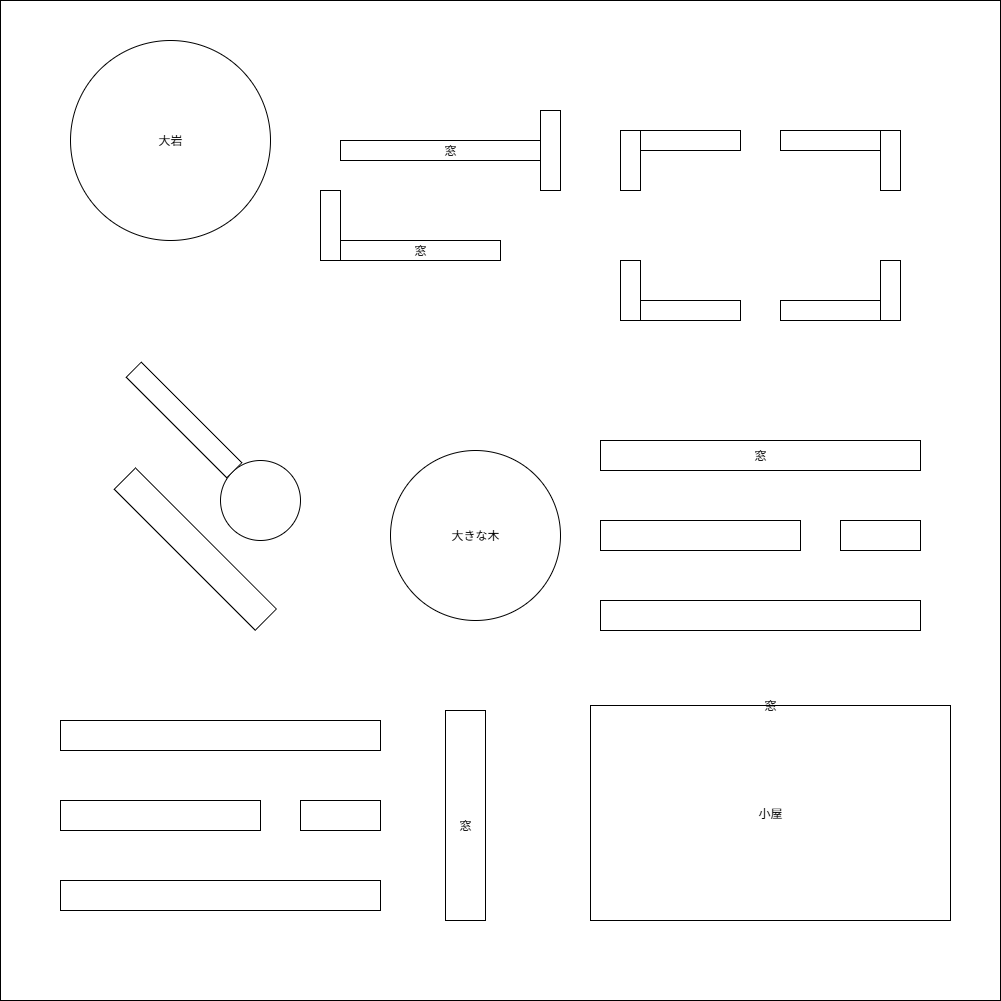
\includegraphics[width=10cm]{MediaEX_試案.png}
    \caption{マップの構造}
    \label{fig:my_label}
\end{figure}


\section{実行結果}
初めに実行結果を示す。
\begin{figure}[H]
    \centering
    \begin{subfigure}[b]{0.48\linewidth}
        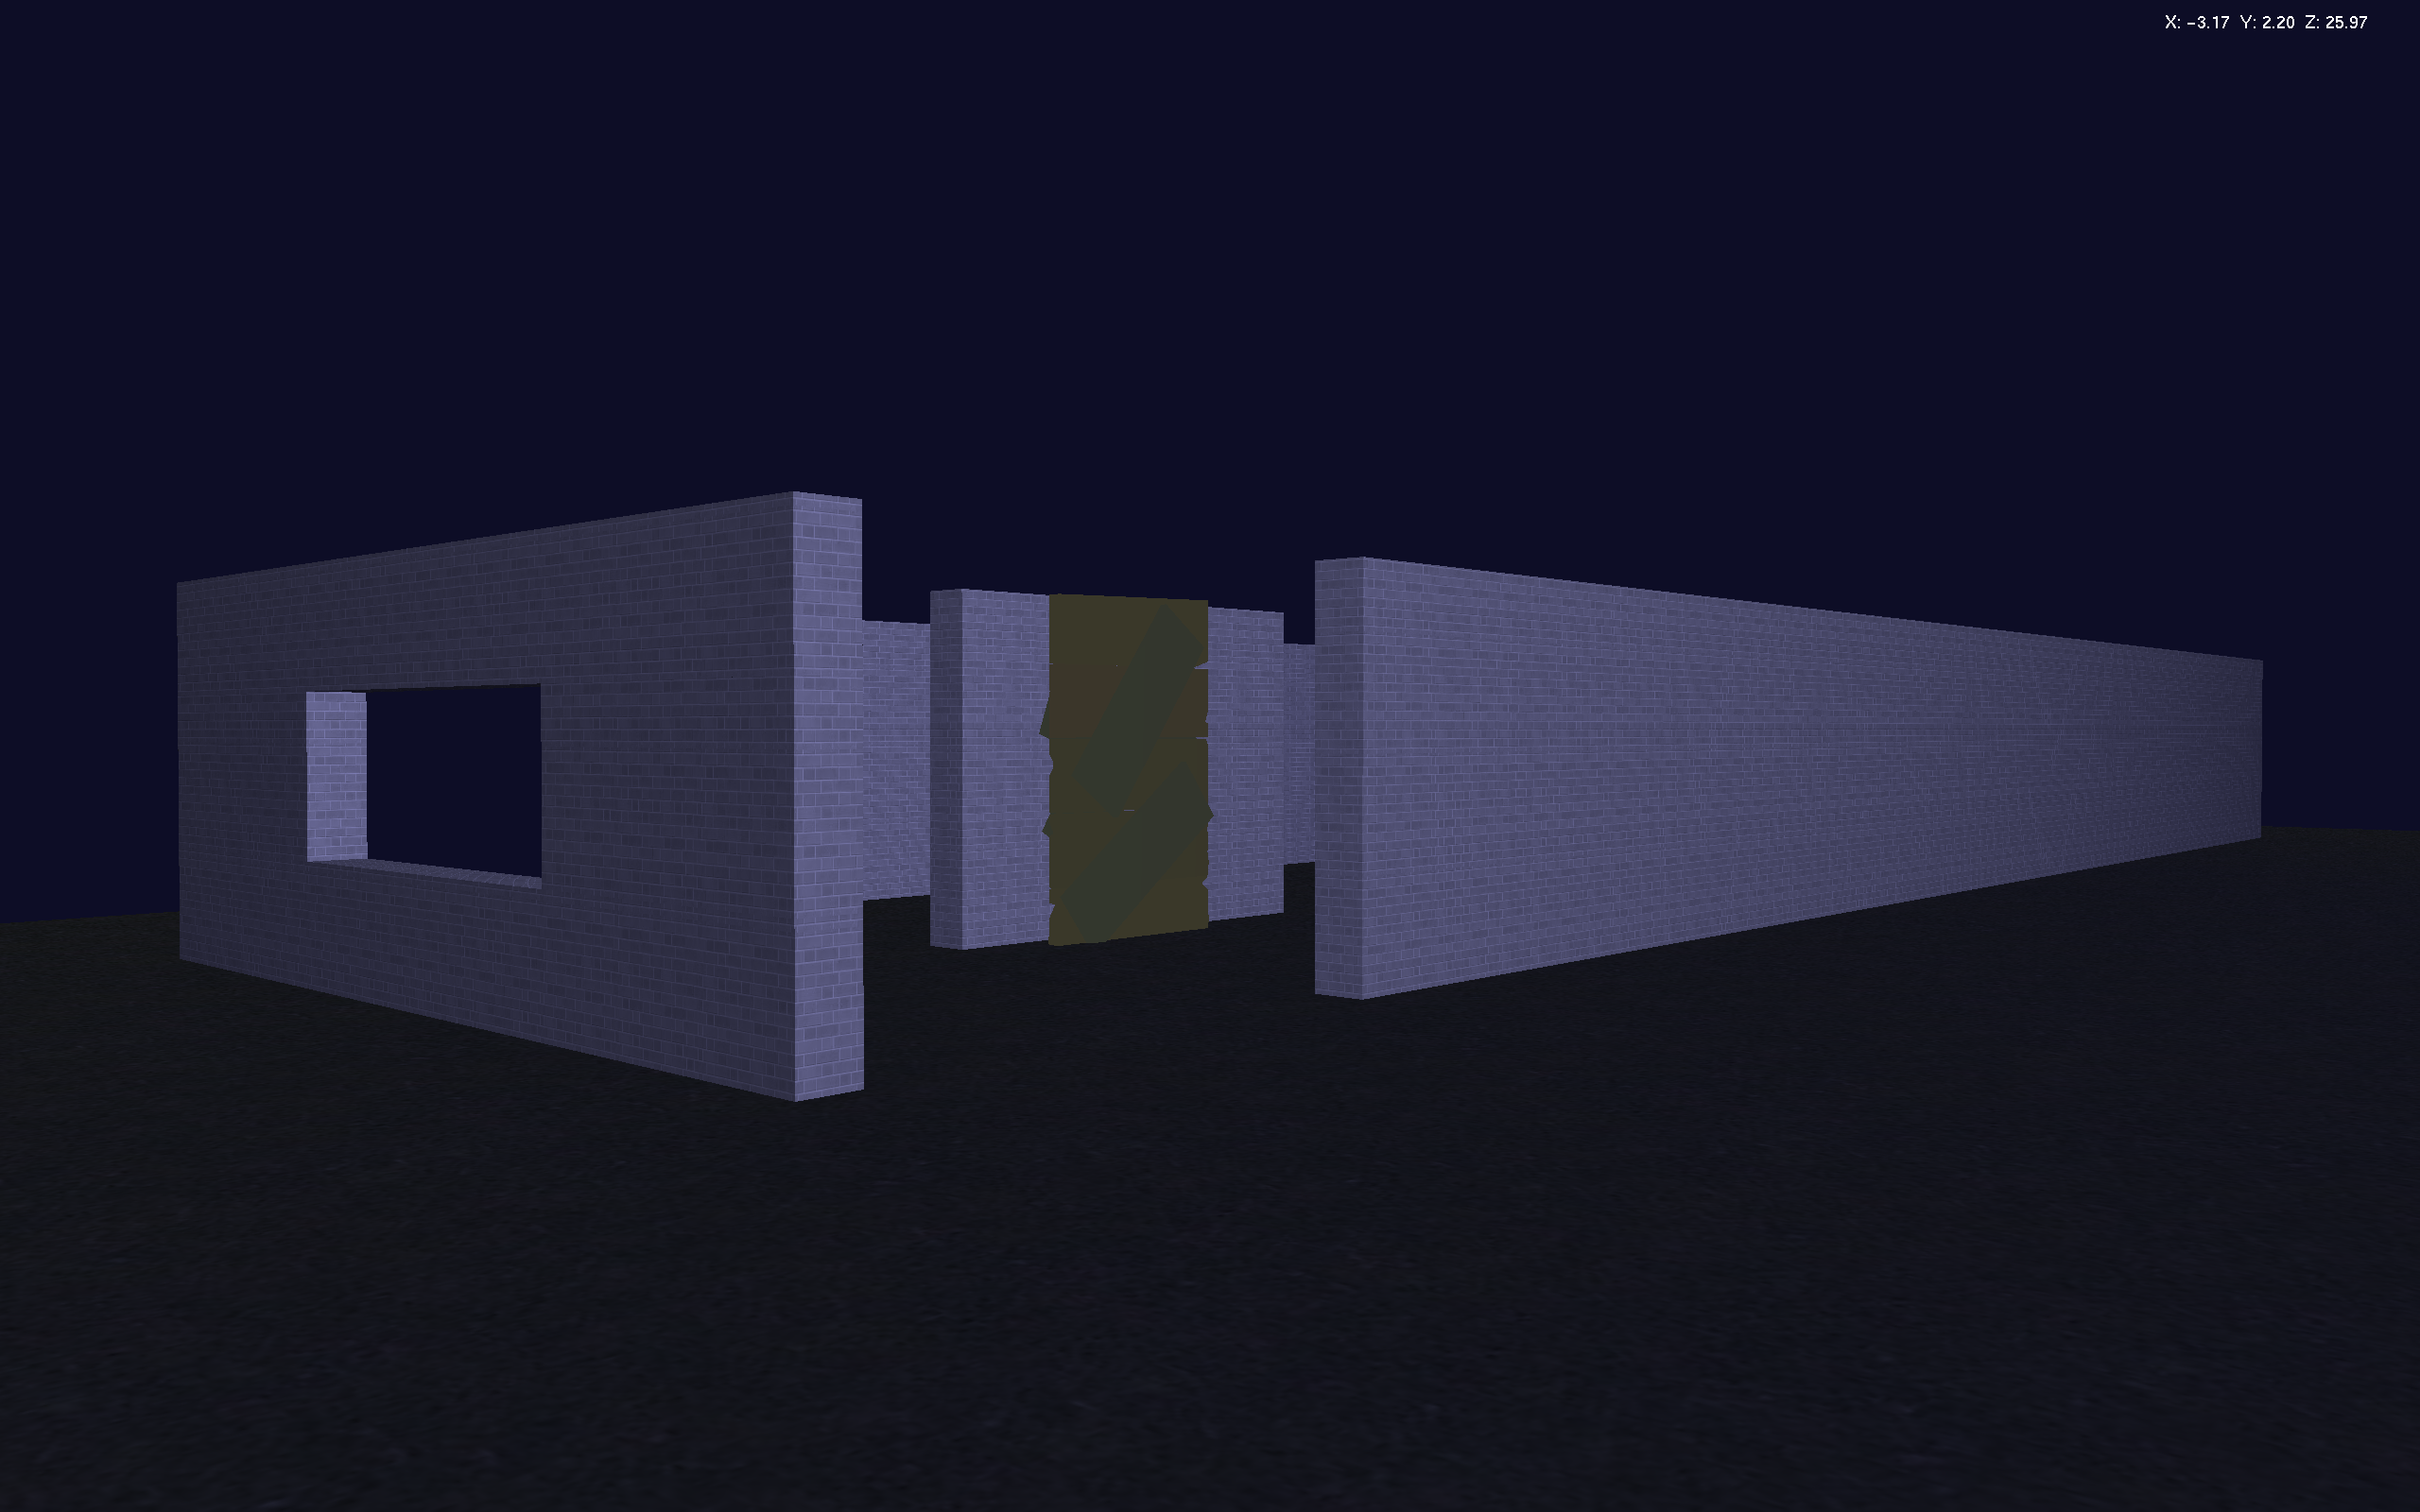
\includegraphics[width=\linewidth]{result1.png}
        \caption{壁とパレット}
        \label{fig:result1}
    \end{subfigure}
    \hfill
    \begin{subfigure}[b]{0.48\linewidth}
        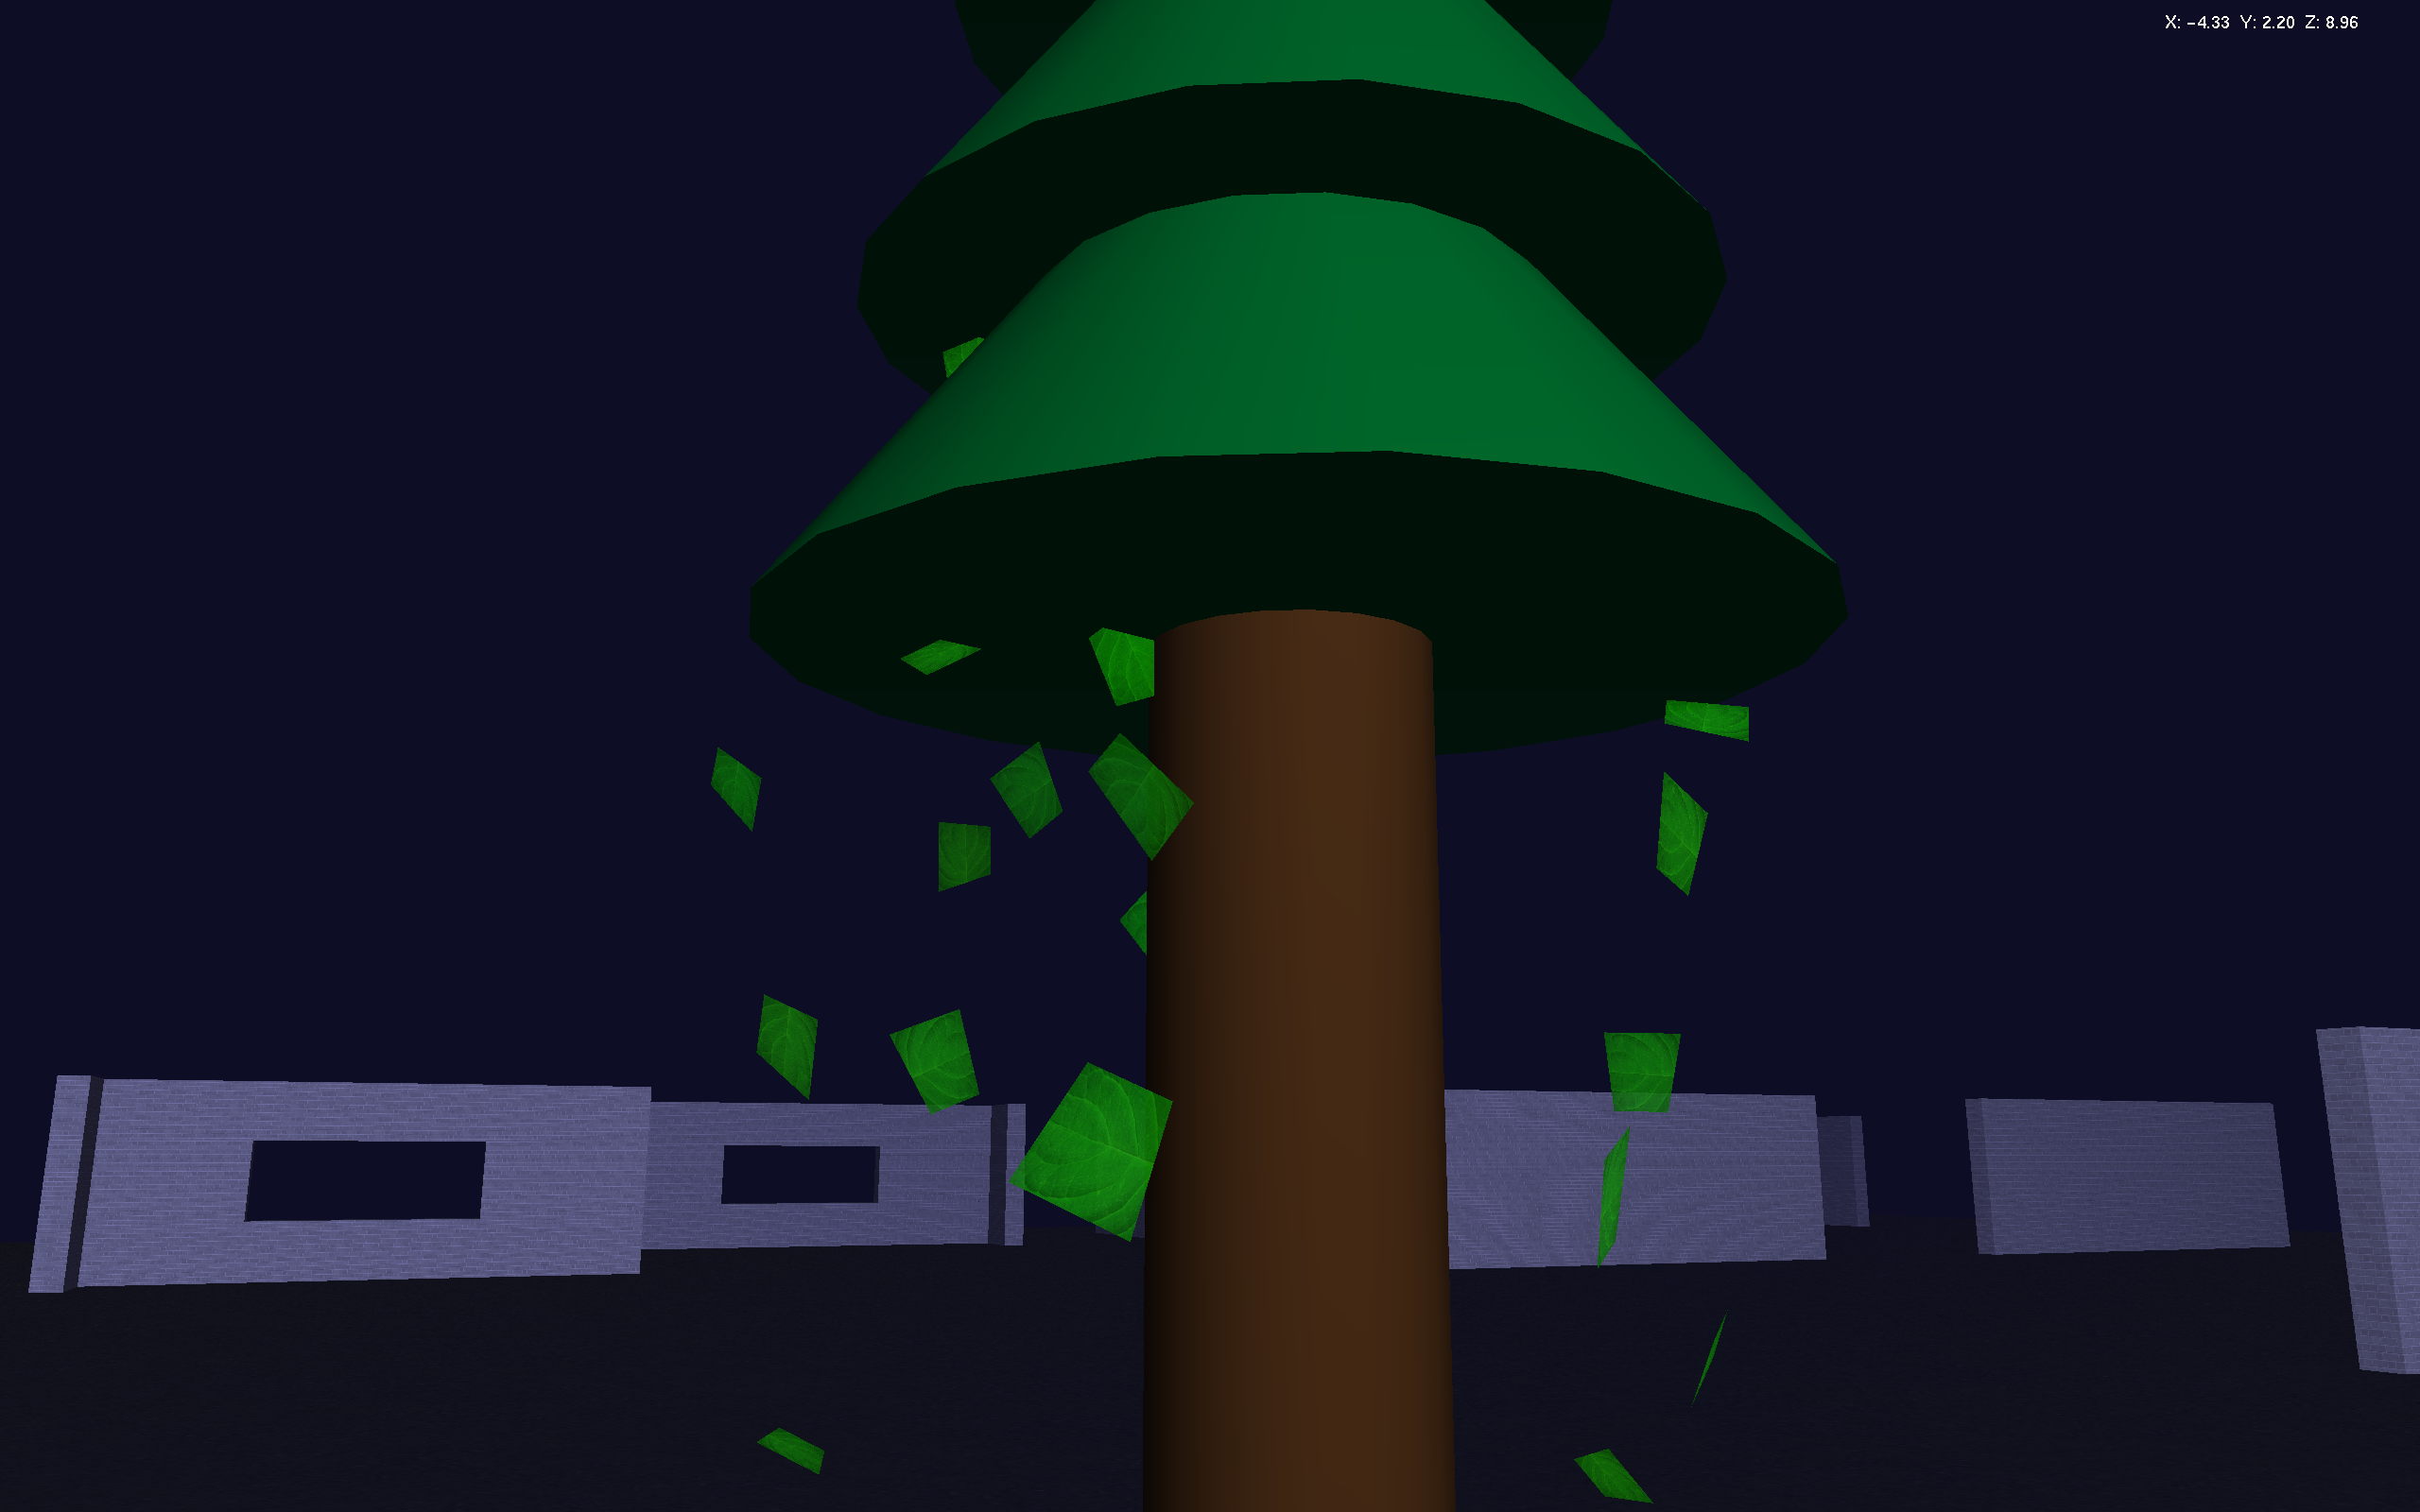
\includegraphics[width=\linewidth]{result2.png}
        \caption{近づくと葉っぱが落ちてくる木}
        \label{fig:result2}
    \end{subfigure}

    \vspace{4mm}

    \begin{subfigure}[b]{0.48\linewidth}
        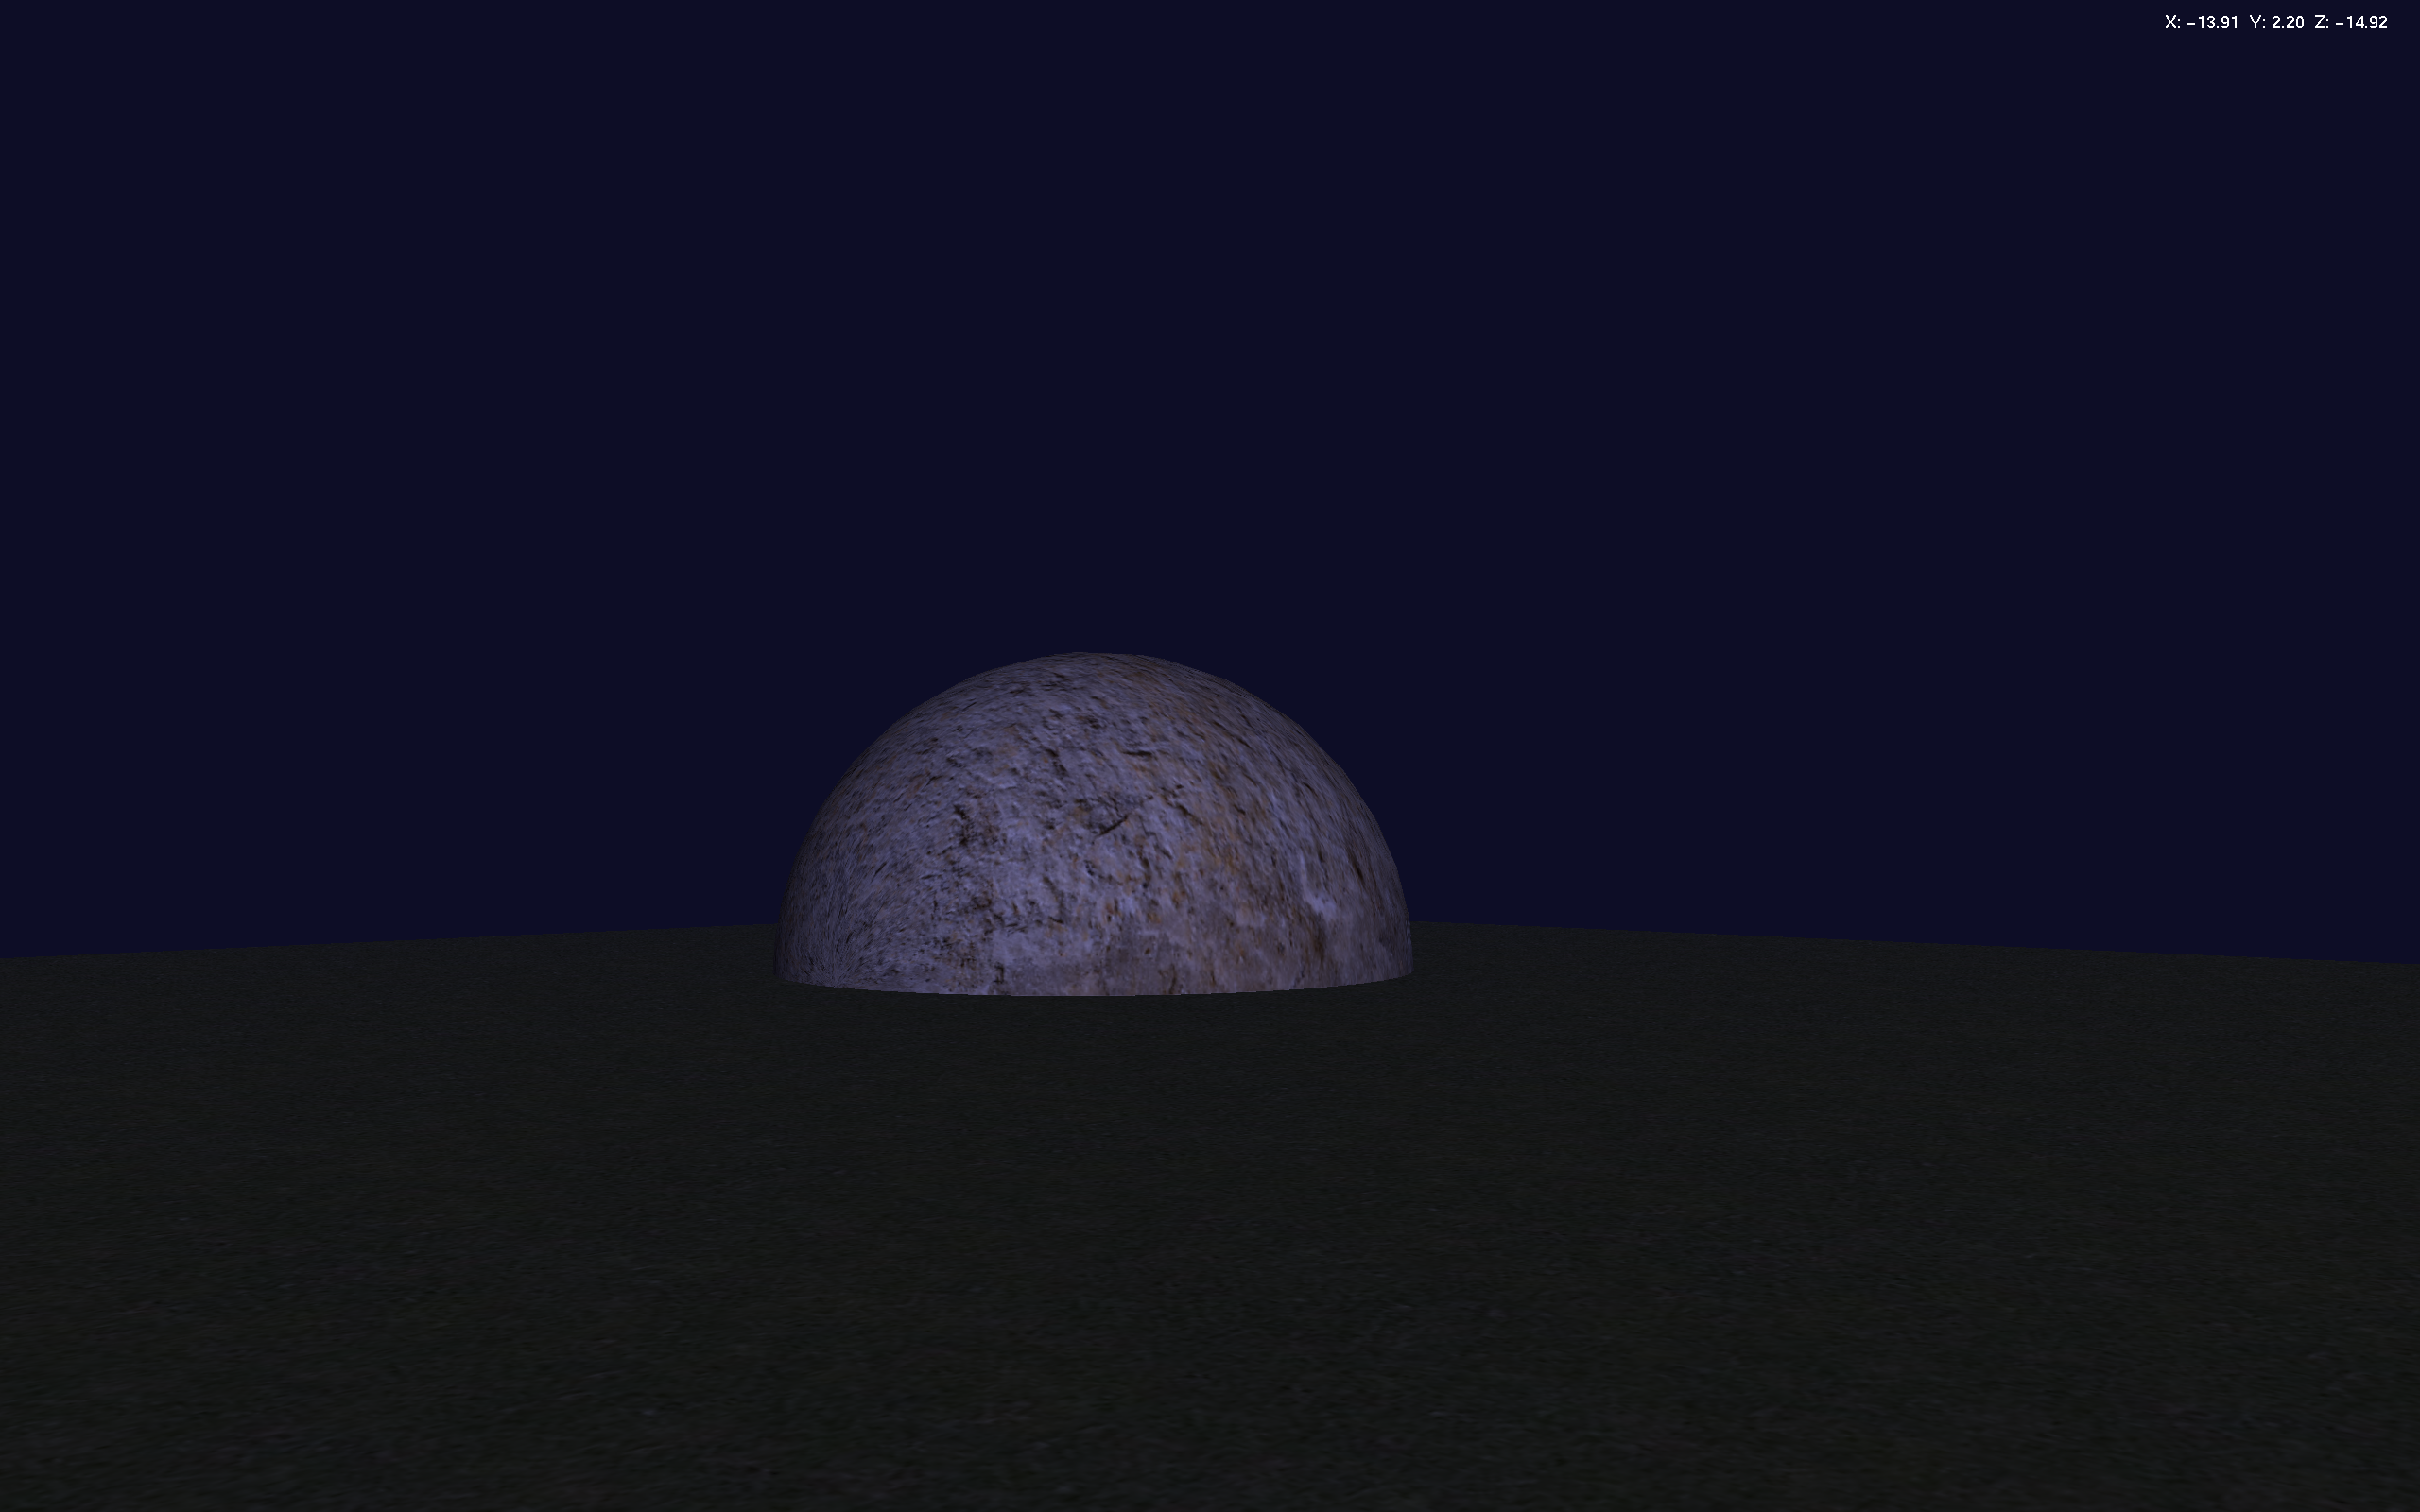
\includegraphics[width=\linewidth]{result3.png}
        \caption{textureを貼り付けた岩}
        \label{fig:result3}
    \end{subfigure}
    \hfill
    \begin{subfigure}[b]{0.48\linewidth}
        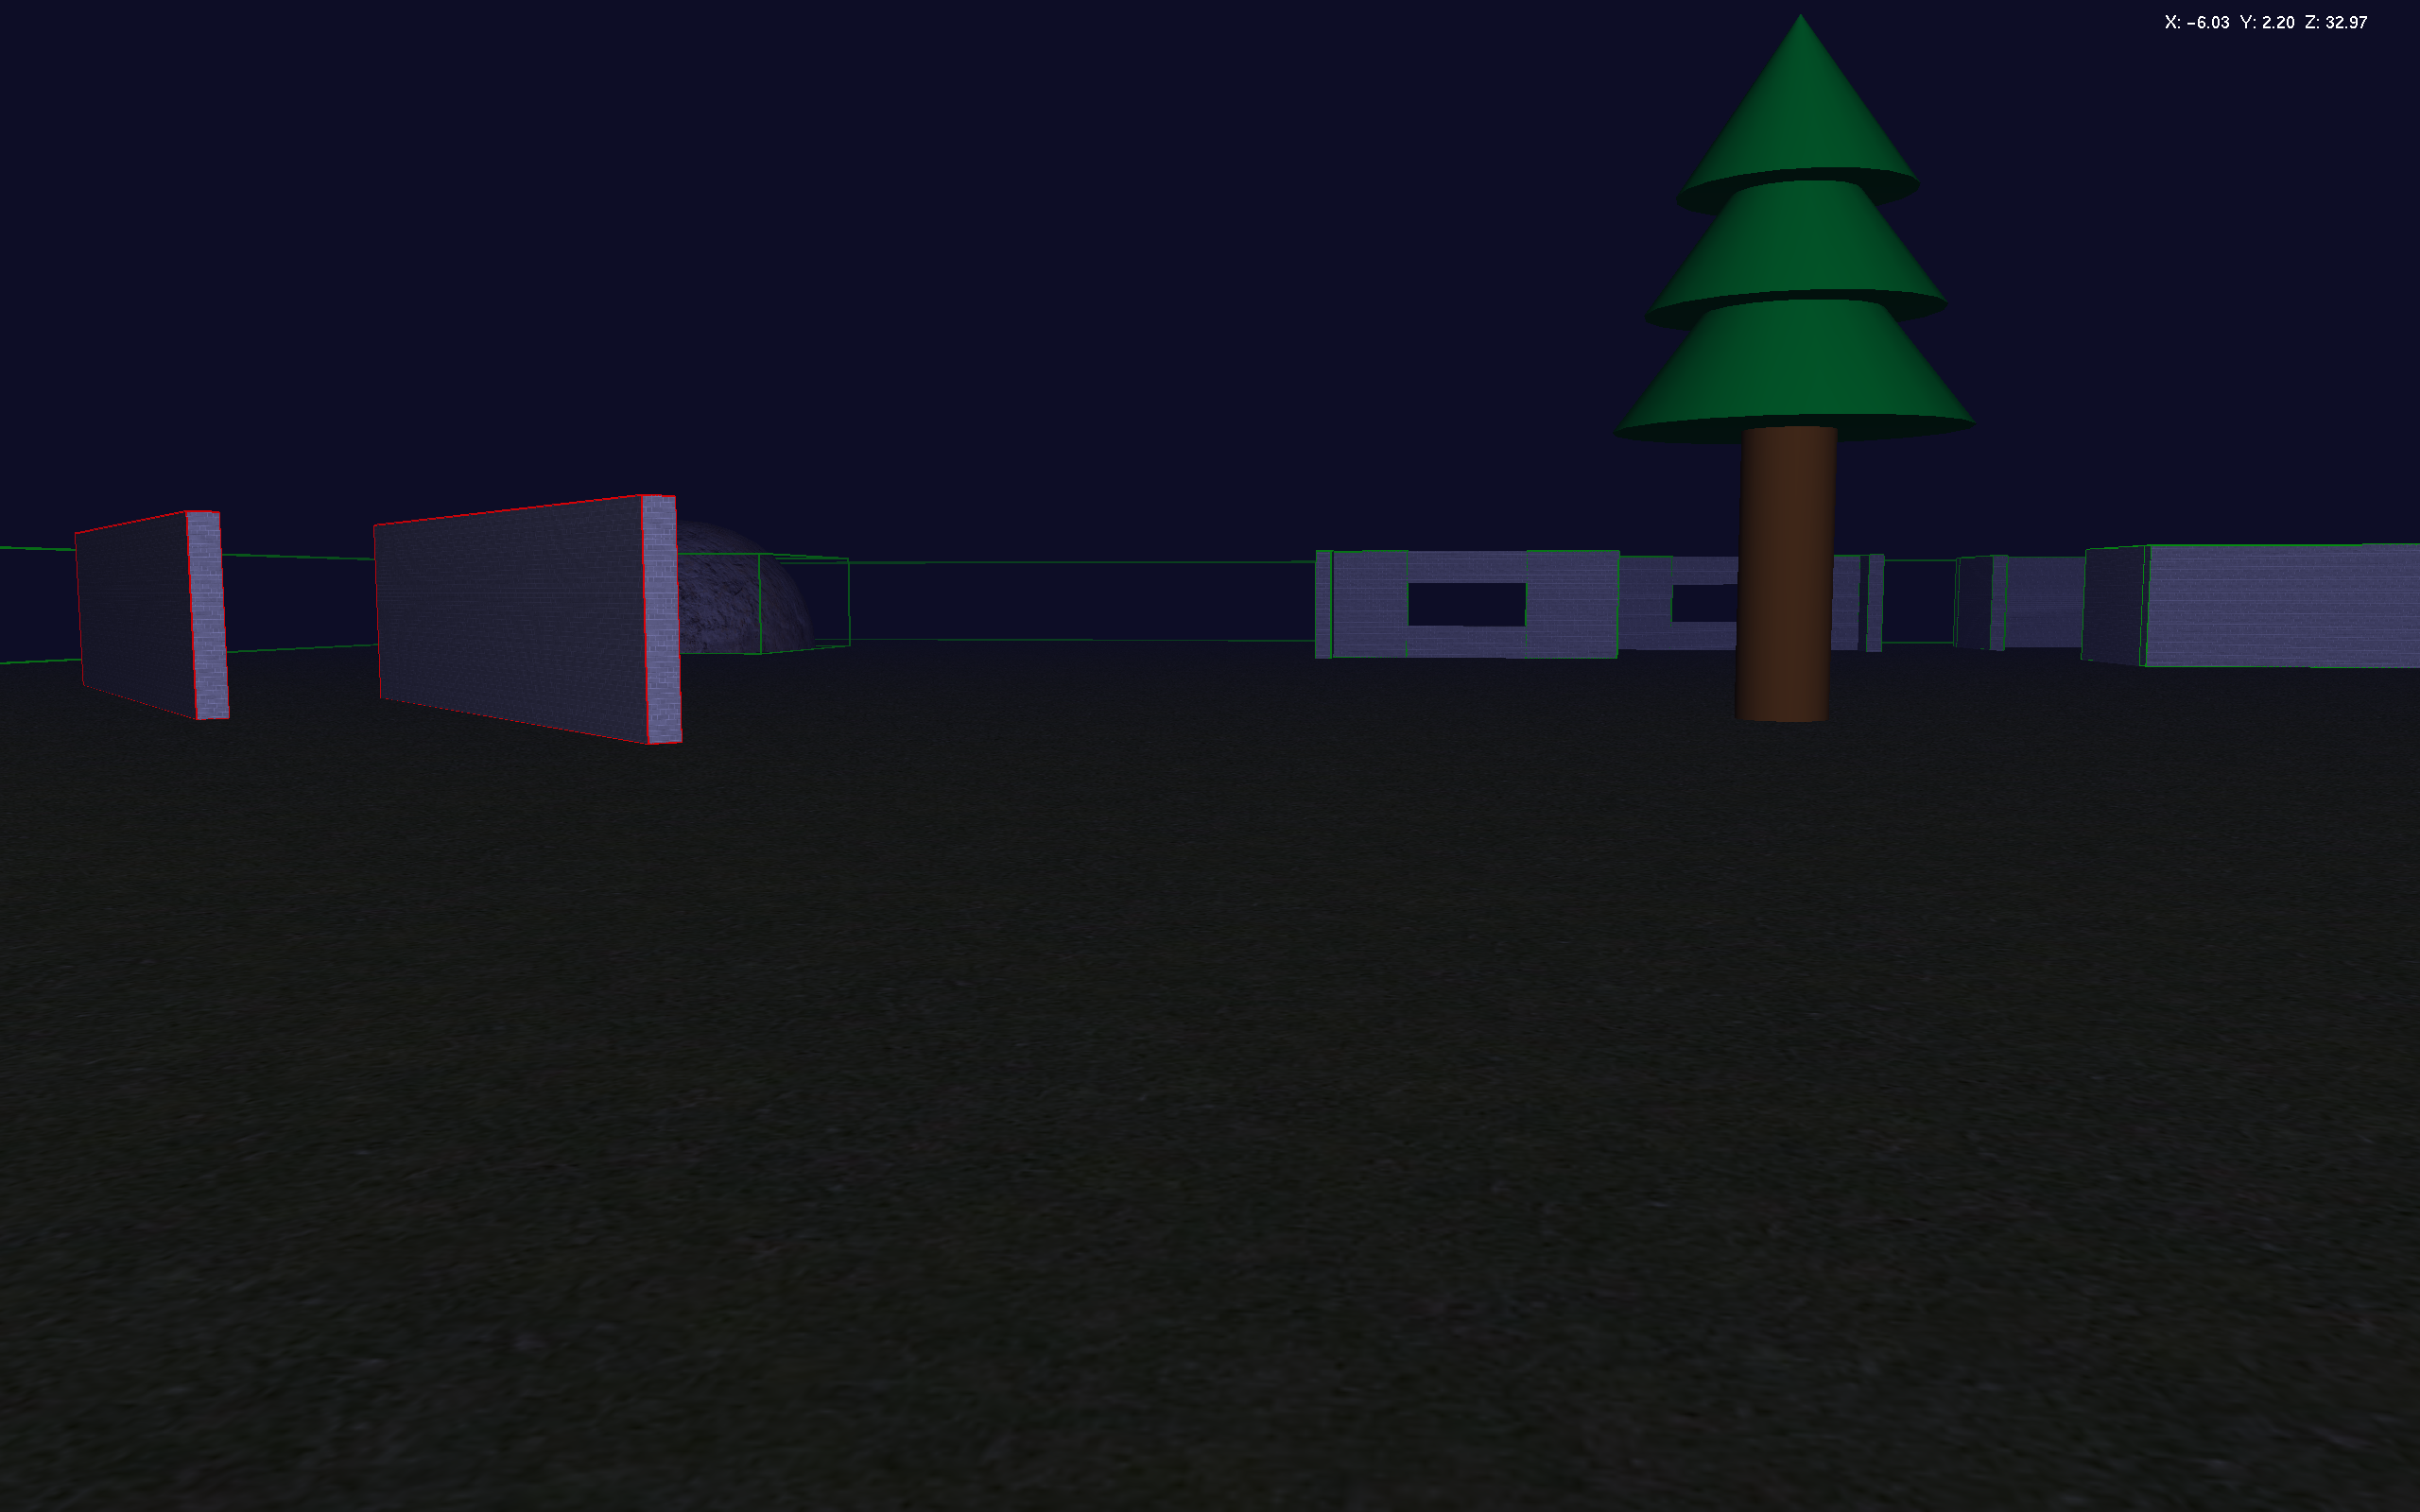
\includegraphics[width=\linewidth]{result4.png}
        \caption{当たり判定の可視化}
        \label{fig:result4}
    \end{subfigure}

    \caption{実行結果(result1〜result4)}
    \label{fig:results}
\end{figure}

\clearpage
\section{コード内容}
\subsection{ヘッダーファイル}
今回読み込んでいるヘッダーファイルは次のとおりである。
\begin{table}[H]
    \centering
    \caption{C++ヘッダファイルと本プログラムにおける用途}
    \label{tab:cpp_headers_intent}
    \begin{tabular}{lp{10cm}}
    \toprule
    \textbf{ヘッダーファイル/マクロ} & \textbf{このプログラムにおける用途} \\
    \midrule
    \texttt{<GL/glut.h>} & \textbf{実験での指定}。ウィンドウの表示、キーボード・マウス入力の受付、描画ループの管理など、アプリケーションの骨格として使用。 \\ \addlinespace
    \texttt{\#define \_USE\_MATH\_DEFINES} & カメラの向きや円運動の計算に必要な円周率の定数 \texttt{M\_PI} を \texttt{<cmath>} 内で有効化するために記述。 \\ \addlinespace
    \texttt{<cmath>} & カメラの向き(三角関数 \texttt{sin}, \texttt{cos})、当たり判定(平方根 \texttt{sqrt})、パーリンノイズ(\texttt{floor})など、3D空間の計算処理全般で使用。 \\ \addlinespace
    \texttt{<vector>} & 壁、パレット、落ち葉など、シーン内に複数存在するオブジェクトのリストを可変長配列として管理するために使用。 \\ \addlinespace
    \texttt{<cstdio>} & \texttt{sprintf} を使い、プレイヤーの現在座標をリアルタイムで文字列に変換し、画面右上のHUDに表示するために使用。 \\ \addlinespace
    \texttt{<cctype>} & \texttt{tolower} を使い、キーボード入力で大文字・小文字を区別せず(例:'W'と'w'を同じ前進命令として)扱うために使用。 \\ \addlinespace
    \texttt{<opencv2/opencv.hpp>} & 地面や壁、岩などに貼り付けるテクスチャ(.jpg画像)をファイルから読み込み、OpenGLで扱える形式に変換するために使用。 \\ \addlinespace
    \texttt{<iostream>} & モデルやテクスチャの読み込みが成功したか、あるいは失敗したかといったプログラムの動作状況をコンソールに出力するために使用。 \\ \addlinespace
    \texttt{<string>} & \texttt{".obj"} や \texttt{".jpg"} ファイルのパスを文字列として扱い、モデルやテクスチャの読み込み関数に渡すために使用。 \\ \addlinespace
    \texttt{<locale.h>} & PCの地域設定に依らず、.objファイル内の小数点を一貫して「.」として読み込ませ、モデルの読み込みエラーを防ぐために使用。 \\ \addlinespace
    \texttt{<random>} & 舞い散る葉の位置・色・回転速度などをランダムに決定し、自然に見えるパーティクルエフェクトを生成するために使用。 \\ \addlinespace
    \texttt{<algorithm>} & 地面に落ちた葉をリストから効率的に削除する(\texttt{std::remove\_if})ため、またパーリンノイズの初期化(\texttt{std::shuffle})のために使用。 \\ \addlinespace
    \texttt{<numeric>} & パーリンノイズの計算に必要な配列を \texttt{0, 1, 2...} という連番で高速に初期化するため(\texttt{std::iota})に使用。 \\ \addlinespace
    \texttt{<limits>} & 当たり判定の内部計算で、比較の初期値として浮動小数点数の最大値を取得するために使用。 \\ \addlinespace
    \texttt{<cstring>} & 自作の透視投影行列の計算関数内で、行列データを効率的にゼロで初期化するため(\texttt{memset})に使用。 \\ \addlinespace
    \texttt{"tiny\_obj\_loader.h"} & ステージに配置されているパレットと家の3Dモデル(.obj形式)をファイルから読み込み、描画可能なデータに変換するために使用。 \\
    \bottomrule
    \end{tabular}
\end{table}

\clearpage
\subsection{グローバル変数}
\begin{longtable}{lll}
    \caption{グローバル変数の役割}
    \label{tab:global_variables_long} \\
    
    \toprule
    \textbf{型} & \textbf{変数名} & \textbf{目的} \\
    \midrule
    \endfirsthead
    
    \multicolumn{3}{l}{\tablename~\thetable{} -- 前ページからの続き} \\
    \toprule
    \textbf{型} & \textbf{変数名} & \textbf{目的} \\
    \midrule
    \endhead
    
    \bottomrule
    \endlastfoot

    % --- 表の内容 ---
    \multicolumn{3}{l}{\textit{--- カメラ・プレイヤー関連 ---}} \\
    \texttt{float} & \texttt{cameraX, cameraY, cameraZ} & プレイヤー(カメラ)の現在位置(X, Y, Z座標)を保持する。 \\
    \texttt{float} & \texttt{yaw, pitch} & プレイヤーの視点の向き(水平・垂直の回転角度)を保持する。 \\
    \texttt{int} & \texttt{lastMouseX, lastMouseY} & マウス視点操作で、前フレームのマウス位置を記憶するために使用。 \\
    \texttt{bool} & \texttt{firstMouse} & マウスがウィンドウに入った直後の視点の急なブレを防ぐためのフラグ。 \\
    \texttt{bool} & \texttt{justWarped} & カーソルを画面中央に強制移動させた直後かを判定するフラグ。 \\
    \texttt{bool} & \texttt{isMouseLookActive} & カーソルがウィンドウ内にある時だけ視点操作を有効にするためのフラグ。 \\
    \addlinespace
    \multicolumn{3}{l}{\textit{--- ウィンドウ・シーン関連 ---}} \\
    \texttt{int} & \texttt{windowWidth, windowHeight} & ウィンドウの現在の幅と高さを保持し、描画範囲の調整に使用。 \\
    \texttt{bool} & \texttt{keyStates[256]} & 全てのキーの押下状態(押されている/いない)を管理する配列。 \\
    \texttt{bool} & \texttt{showColliders} & デバッグ用に当たり判定のワイヤーフレーム表示を切り替えるフラグ。 \\
    \texttt{GLuint} & \texttt{...TextureID} & OpenGLで管理される各テクスチャ(地面、壁など)の識別番号を保持。 \\
    \texttt{float} & \texttt{g\_time} & プログラム開始からの経過時間を保持し、アニメーションの同期に使用。 \\
    \addlinespace
    \multicolumn{3}{l}{\textit{--- オブジェクト・当たり判定関連 ---}} \\
    \texttt{Model} & \texttt{paletModel, blenderModel} & 読み込んだ3Dモデルの頂点や材質データを保持する。 \\
    \texttt{vector<BoundingBox>} & \texttt{wallColliders} & 壁などの動かないオブジェクトの当たり判定(AABB)情報を管理。 \\
    \texttt{vector<OBB>} & \texttt{obbColliders} & 回転を考慮する当たり判定(OBB)情報を管理。 \\
    \texttt{vector<Pallet>} & \texttt{pallets} & シーン内の全パレットの位置、回転、状態などをリストで管理。 \\
    \texttt{vector<Leaf>} & \texttt{fallingLeaves} & 表示中の全葉パーティクルの状態をリストで管理。 \\
\end{longtable}

\clearpage
\subsection{関数}
\subsubsection{関数一覧}
はじめに今回作成した関数の概要をまとめる。
\begin{longtable}{lp{0.7\textwidth}}
    \caption{関数とその目的}
    \label{tab:functions_long} \\

    \toprule
    \textbf{関数名} & \textbf{目的} \\
    \midrule
    \endfirsthead

    \multicolumn{2}{l}{\tablename~\thetable{} -- 前ページからの続き} \\
    \toprule
    \textbf{関数名} & \textbf{目的} \\
    \midrule
    \endhead

    \bottomrule
    \endlastfoot

    % --- 表の内容 ---
    \multicolumn{2}{l}{\textit{--- 数学ヘルパー関数 ---}} \\
    \texttt{\hyperlink{func:cross}{cross()}} & 3Dベクトルの外積を計算する。カメラの向きの計算で使用。 \\
    \texttt{\hyperlink{func:dot}{dot()}} & 3D/2Dベクトルの内積を計算する。当たり判定やカメラ計算で使用。 \\
    \texttt{\hyperlink{func:normalize}{normalize()}} & 3Dベクトルの長さを1に正規化する。カメラの向きの計算で使用。 \\
    \texttt{\hyperlink{func:perspectiveMatrix}{perspectiveMatrix()}} & 透視投影行列を自前で作成する。 \\
    \texttt{\hyperlink{func:lookAtMatrix}{lookAtMatrix()}} & カメラの位置と注視点からビュー行列を自前で作成する。 \\
    \texttt{\hyperlink{func:drawTexturedSphere}{drawTexturedSphere()}} & テクスチャ付きの球体を自前で描画する。 \\
    \addlinespace
    \multicolumn{2}{l}{\textit{--- パーリンノイズ関連関数 ---}} \\
    \texttt{\hyperlink{func:perlin_helpers}{fade(), linearInterpolate(), grad()}} & パーリンノイズの値を滑らかに補間するための計算用ヘルパー関数。 \\
    \texttt{\hyperlink{func:initPerlinNoise}{initPerlinNoise()}} & パーリンノイズ生成に必要なランダムな変換テーブルを最初に一度だけ作成する。 \\
    \texttt{\hyperlink{func:perlinNoise}{perlinNoise()}} & 指定された3次元座標に対応するノイズ値を生成し、葉の揺らぎに使用。 \\
    \addlinespace
    \multicolumn{2}{l}{\textit{--- モデル・テクスチャ処理関数 ---}} \\
    \texttt{\hyperlink{func:calculateModelBBox}{calculateModelBBox()}} & .objモデルの全頂点を調査し、モデルを囲む最小の箱(バウンディングボックス)を計算。 \\
    \texttt{\hyperlink{func:loadObjModel}{loadObjModel()}} & tinyobjloaderを使い、.obj形式の3Dモデルファイルを読み込んでデータ構造に格納する。 \\
    \texttt{\hyperlink{func:drawObjModel}{drawObjModel()}} & 読み込んだ3Dモデルを指定された設定で描画する。発光効果にも対応。 \\
    \texttt{\hyperlink{func:loadTexture}{loadTexture()}} & OpenCVを使い、画像ファイルを読み込んでOpenGLのテクスチャとして利用可能にする。 \\
    \addlinespace
    \multicolumn{2}{l}{\textit{--- 描画関連関数 ---}} \\
    \texttt{\hyperlink{func:renderBitmapString}{renderBitmapString()}} & 画面上の指定座標にデバッグ情報などの文字列を描画する。 \\
    \texttt{\hyperlink{func:drawHUD}{drawHUD()}} & 画面右上にプレイヤーの現在座標をオーバーレイ表示する。 \\
    \texttt{\hyperlink{func:drawGround}{drawGround()}} & シーンの土台となる地面を描画する。 \\
    \texttt{\hyperlink{func:drawWalls}{drawWalls()}} & ステージを構成する全ての壁を描画する。 \\
    \texttt{\hyperlink{func:drawTree}{drawTree()}} & 円柱と円錐を組み合わせた木を描画する。 \\
    \texttt{\hyperlink{func:drawRock}{drawRock()}} & テクスチャ付きの球体で岩を描画する。 \\
    \texttt{\hyperlink{func:drawCylinder}{drawCylinder()}} & 木の幹などを描画するために使用する円柱の描画関数。 \\
    \texttt{\hyperlink{func:drawFallingLeaves}{drawFallingLeaves()}} & 葉のパーティクルエフェクトを描画する。 \\
    \texttt{\hyperlink{func:drawColliders}{drawColliders()}} & デバッグ用に当たり判定領域をワイヤーフレームで可視化する。 \\
    \addlinespace
    \multicolumn{2}{l}{\textit{--- 初期化・状態更新関数 ---}} \\
    \texttt{\hyperlink{func:setupColliders}{setupColliders()}} & 壁やオブジェクトの当たり判定をプログラム開始時にセットアップする。 \\
    \texttt{\hyperlink{func:setupPallets}{setupPallets()}} & パレットオブジェクトを初期位置に配置する。 \\
    \texttt{\hyperlink{func:updatePallets}{updatePallets()}} & パレットの浮遊アニメーションやインタラクション後の状態を更新する。 \\
    \texttt{\hyperlink{func:spawnLeaf}{spawnLeaf()}} & 新しい葉パーティクルをランダムな設定で生成する。 \\
    \texttt{\hyperlink{func:updateFallingLeaves}{updateFallingLeaves()}} & 全ての葉パーティクルの状態をフレーム毎に更新し、不要なものを消去する。 \\
    \texttt{\hyperlink{func:checkAABBCollision}{checkAABBCollision()}} & プレイヤーとAABB(軸並行な箱)との当たり判定を計算し、衝突解決を行う。 \\
    \texttt{\hyperlink{func:checkOBBCollision}{checkOBBCollision()}} & プレイヤーとOBB(回転した箱)との当たり判定を計算し、衝突解決を行う。 \\
    \addlinespace
    \multicolumn{2}{l}{\textit{--- GLUTコールバック関数 ---}} \\
    \texttt{\hyperlink{func:display}{display()}} & 画面の再描画時に呼び出され、全ての描画命令を発行するメイン描画関数。 \\
    \texttt{\hyperlink{func:update}{update()}} & 一定時間ごとに呼び出され、プレイヤーの位置、アニメーションなどゲーム全体のロジックを更新。 \\
    \texttt{\hyperlink{func:keyboard}{keyboard()}} & キーの押下を検知し、プレイヤーの移動や機能のON/OFFを行う。 \\
    \texttt{\hyperlink{func:keyboardUp}{keyboardUp()}} & キーの解放を検知し、プレイヤーの移動停止を処理する。 \\
    \texttt{\hyperlink{func:mouseMotion}{mouseMotion()}} & マウスの動きを検知し、プレイヤーの視点移動に反映させる。 \\
    \texttt{\hyperlink{func:reshape}{reshape()}} & ウィンドウサイズ変更時に呼び出され、描画のアスペクト比などを再設定する。 \\
    \texttt{\hyperlink{func:entry}{entry()}} & マウスカーソルの出入りを検知し、視点操作の有効/無効を切り替える。 \\
    \texttt{\hyperlink{func:initScene}{initScene()}} & プログラム起動時に一度だけ呼び出され、シーン全体の初期設定を行う。 \\
    \addlinespace
    \multicolumn{2}{l}{\textit{--- メイン関数 ---}} \\
    \texttt{\hyperlink{func:main}{main()}} & プログラムのエントリーポイント。GLUTの初期化とウィンドウ作成、コールバック関数の登録を行う。 \\
\end{longtable}

\clearpage
ここから1つ1つの関数について説明を行う。

\hypertarget{func:cross}{}\subsubsection{cross()}\label{func:cross}
\begin{lstlisting}[language=C++, caption={cross() 関数}, label={lst:cross_detail}]
/**
 * @brief ベクトルの外積を計算する。
 * @param a 1ベクトル
 * @param b 2ベクトル
 * @return 外積ベクトル
 */
Vec3 cross(const Vec3& a, const Vec3& b) {
    return {a.y * b.z - a.z * b.y, a.z * b.x - a.x * b.z, a.x * b.y - a.y * b.x};
}
\end{lstlisting}
この関数では、2つの3Dベクトルに対する外積を計算している。
特にlookAtMatrixというカメラ制御関数において右方向と上方向を決定するときに使用するヘルプ関数である。
例えば、カメラの正面の向きと上の向きの外積を計算することにより、右方向が決定できる。

\hypertarget{func:dot}{}\subsubsection{dot()}\label{func:dot}
\begin{lstlisting}[language=C++, caption={dot() 関数 (3Dベクトル版)}, label={lst:dot_detail}]
/**
 * @brief 内積を計算する。
 * @param a 1ベクトル
 * @param b 2ベクトル
 * @return ベクトルの内積
 */
float dot(const Vec3& a, const Vec3& b) {
    return a.x * b.x + a.y * b.y + a.z * b.z;
}
\end{lstlisting}
この関数では、2つの3Dベクトルに対する内積を計算している。
このプログラムでは、ベクトルの長さを決めるときや、カメラの位置を決定するときにdot関数を使っている。

\hypertarget{func:normalize}{}\subsubsection{normalize()}\label{func:normalize}
\begin{lstlisting}[language=C++, caption={normalize() 関数}, label={lst:normalize_detail}]
/**
 * @brief ベクトルを正規化する。
 * @param v 正規化するベクトル
 * @return 正規化されたベクトル
 */
Vec3 normalize(const Vec3& v) {
    float len = std::sqrt(dot(v, v));
    if (len > 0) {
        return {v.x / len, v.y / len, v.z / len};
    }
    return v;
}
\end{lstlisting}
この関数はベクトルの正規化を行う関数である。
三平方の定理を用いてベクトルの長さを計算し、その結果で割っている。
この関数は、lookAtMatrix()の中で、カメラの向きを定義する軸ベクトルを単位ベクトルにそろえるために使用している。

\hypertarget{func:perspectiveMatrix}{}\subsubsection{perspectiveMatrix()}\label{func:perspectiveMatrix}
\begin{lstlisting}[language=C++, caption={perspectiveMatrix() 関数}, label={lst:perspectiveMatrix_detail}]
/**
 * @brief 透視投影行列を作成する。
 * @param mat 結果を格納する配列
 * @param fovY 視野角 (度数法)
 * @param aspect アスペクト比 (幅 / 高さ)
 * @param zNear 前方クリッピング面までの距離
 * @param zFar 後方クリッピング面までの距離
 */
void perspectiveMatrix(float* mat, float fovY, float aspect, float zNear, float zFar) {
    memset(mat, 0, 16 * sizeof(float));
    float f = 1.0f / tanf(fovY * (M_PI / 180.0f) / 2.0f);
    mat[0] = f / aspect;
    mat[5] = f;
    mat[10] = (zFar + zNear) / (zNear - zFar);
    mat[11] = -1.0f;
    mat[14] = (2.0f * zFar * zNear) / (zNear - zFar);
}
\end{lstlisting}
この関数は3D空間を2Dの画面に映し出すための透視投影行列を作成するものである。
forYは視野角を、aspectはアスペクト比を。zNearとzFarて描画範囲を設定している。
この関数はreshape()で使用している。特に視点移動で苦労した際に追加した。
現在はフルスクリーンを固定にしているため、実際に動くことは少ないが、フルスクリーン設定を解除したときにreshapeにてウィンドウサイズが変更されたときに呼び出される。

\hypertarget{func:lookAtMatrix}{}\subsubsection{lookAtMatrix()}\label{func:lookAtMatrix}
\begin{lstlisting}[language=C++, caption={lookAtMatrix() 関数}, label={lst:lookAtMatrix_detail}]
/**
 * @brief ビュー行列を作成する。
 * @param mat 結果を格納する配列
 * @param eye カメラの位置
 * @param center 注視点
 * @param up カメラの上方向
 */
void lookAtMatrix(float* mat, const Vec3& eye, const Vec3& center, const Vec3& up) {
    Vec3 f = normalize({center.x - eye.x, center.y - eye.y, center.z - eye.z});
    Vec3 s = normalize(cross(f, up));
    Vec3 u = cross(s, f);
    mat[0] = s.x; mat[4] = s.y; mat[8] = s.z; mat[12] = -dot(s, eye);
    mat[1] = u.x; mat[5] = u.y; mat[9] = u.z; mat[13] = -dot(u, eye);
    mat[2] = -f.x; mat[6] = -f.y; mat[10] = -f.z; mat[14] = dot(f, eye);
    mat[3] = 0.0f; mat[7] = 0.0f; mat[11] = 0.0f; mat[15] = 1.0f;
}
\end{lstlisting}
この関数は、3D空間における仮想的なカメラの位置と向きを定義するための関数である。
今回の視点移動はカメラを動かすのではなく、3D空間全てのオブジェクトを動かすことで、あたかもカメラが移動しているかのように錯覚させて、実装している。
この関数はフレームごとの描画を行うdisplay()関数にて使用している。

\hypertarget{func:drawTexturedSphere}{}\subsubsection{drawTexturedSphere()}\label{func:drawTexturedSphere}
\begin{lstlisting}[language=C++, caption={drawTexturedSphere() 関数}, label={lst:drawTexturedSphere_detail}]
/**
 * @brief テクスチャマッピング可能な球体を描画する。
 * @param radius 球の半径
 * @param slices 経度方向の分割数
 * @param stacks 緯度方向の分割数
 */
void drawTexturedSphere(GLdouble radius, GLint slices, GLint stacks) {
    for (int i = 0; i < stacks; ++i) {
        GLdouble lat0 = M_PI * (-0.5 + (double)i / stacks);
        GLdouble z0 = radius * sin(lat0);
        GLdouble zr0 = radius * cos(lat0);
        GLdouble lat1 = M_PI * (-0.5 + (double)(i + 1) / stacks);
        GLdouble z1 = radius * sin(lat1);
        GLdouble zr1 = radius * cos(lat1);
        glBegin(GL_QUAD_STRIP);
        for (int j = 0; j <= slices; ++j) {
            GLdouble lng = 2 * M_PI * (double)j / slices;
            GLdouble x = cos(lng);
            GLdouble y = sin(lng);
            glNormal3d(x * zr1, y * zr1, z1);
            glTexCoord2d((double)j / slices, (double)(i + 1) / stacks);
            glVertex3d(x * zr1, y * zr1, z1);
            glNormal3d(x * zr0, y * zr0, z0);
            glTexCoord2d((double)j / slices, (double)i / stacks);
            glVertex3d(x * zr0, y * zr0, z0);
        }
        glEnd();
    }
}
\end{lstlisting}
この関数では、textureを貼り付けることができる3Dの球体を作成する。
特に大きな岩を作成するときに使用した。

\hypertarget{func:perlin_helpers}{}\subsubsection{fade(), linearInterpolate(), grad()}\label{func:perlin_helpers}
\begin{lstlisting}[language=C++, caption={パーリンノイズ用ヘルパー関数}, label={lst:perlin_helpers_detail}]
/**
 * @brief パーリンノイズで滑らかな補間を行うためのフェード関数。
 * @param t 入力値
 * @return 補間された値
 */
float fade(float t) { return t * t * t * (t * (t * 6 - 15) + 10); }

/**
 * @brief 線形補間を行う。
 * @param a 開始値
 * @param b 終了値
 * @param t 補間係数
 * @return 補間された値
 */
float linearInterpolate(float a, float b, float t) { return a + t * (b - a); }

/**
 * @brief ハッシュ値に基づいて勾配ベクトルを計算する。
 * @param hash ハッシュ値
 * @param x x座標
 * @param y y座標
 * @param z z座標
 * @return 勾配ベクトルの計算結果
 */
float grad(int hash, float x, float y, float z) {
    int h = hash & 15;
    float u = h < 8 ? x : y;
    float v = h < 4 ? y : (h == 12 || h == 14 ? x : z);
    return ((h & 1) == 0 ? u : -u) + ((h & 2) == 0 ? v : -v);
}
\end{lstlisting}
これらの関数群はparlinNoize()関数の実装のために作ったヘルパー関数である。
fade()はパーリンノイズにて滑らかな保管を行うための関数である。
linearInterpolate()は線形補完を行うための関数である。
grad()はハッシュ値に基づいて勾配ベクトルを計算するための関数である。
詳細はparlinNoise()にて説明する。

\hypertarget{func:initPerlinNoise}{}\subsubsection{initPerlinNoise()}\label{func:initPerlinNoise}
\begin{lstlisting}[language=C++, caption={initPerlinNoise() 関数}, label={lst:initPerlinNoise_detail}]
/**
 * @brief パーリンノイズ生成器を初期化する。ランダムな置換テーブルを作成する。
 */
void initPerlinNoise() {
    std::iota(p, p + 256, 0);
    std::shuffle(p, p + 256, rng);
    for (int i = 0; i < 256; ++i) {
        p[i + 256] = p[i];
    }
}
\end{lstlisting}
この関数はパーリンノイズを作成するために不可欠な置換テーブルという乱数リストの作成を行うものである。
update()と並列処理をすると、この処理が重くカクカクしてしまったので、起動時に呼び出すようにした。

\hypertarget{func:perlinNoise}{}\subsubsection{perlinNoise()}\label{func:perlinNoise}
\begin{lstlisting}[language=C++, caption={perlinNoise() 関数}, label={lst:perlinNoise_detail}]
/**
 * @brief パーリンノイズを生成する。
 * @param x x座標
 * @param y y座標
 * @param z z座標
 * @return ノイズ値
 */
float perlinNoise(float x, float y, float z) {
    int X = (int)floor(x) & 255;
    int Y = (int)floor(y) & 255;
    int Z = (int)floor(z) & 255;
    x -= floor(x);
    y -= floor(y);
    z -= floor(z);
    float u = fade(x), v = fade(y), w = fade(z);
    int A = p[X] + Y, AA = p[A] + Z, AB = p[A + 1] + Z;
    int B = p[X + 1] + Y, BA = p[B] + Z, BB = p[B + 1] + Z;
    float res = linearInterpolate(
        linearInterpolate(
            linearInterpolate(grad(p[AA], x, y, z), grad(p[BA], x - 1, y, z), u),
            linearInterpolate(grad(p[AB], x, y - 1, z), grad(p[BB], x - 1, y - 1, z), u), v),
        linearInterpolate(
            linearInterpolate(grad(p[AA + 1], x, y, z - 1), grad(p[BA + 1], x - 1, y, z - 1), u),
            linearInterpolate(grad(p[AB + 1], x, y - 1, z - 1), grad(p[BB + 1], x - 1, y - 1, z - 1), u), v), w);
    return (res + 1.0f) / 2.0f;
}
\end{lstlisting}
この関数は、パーリンノイズを生成するための関数である。
パーリンノイズとは、通常のrand()と異なり、隣り合う値との関連性がある乱数となる。そのため雲の模様、地形、炎の揺らめきといった、CGにおける様々な自然現象をリアルに表現することに使われている。
パーリンノイズを葉っぱを揺らすために使用している。

\hypertarget{func:calculateModelBBox}{}\subsubsection{calculateModelBBox()}\label{func:calculateModelBBox}
\begin{lstlisting}[language=C++, caption={calculateModelBBox() 関数}, label={lst:calculateModelBBox_detail}]
/**
 * @brief モデルの頂点データから軸並行境界ボックスを計算する。
 * @param model バウンディングボックスを計算するモデル
 * @return 計算されたBoundingBox
 */
BoundingBox calculateModelBBox(const Model& model) {
    if (model.attrib.vertices.empty()) { return {0,0,0,0,0,0}; }
    float minX = model.attrib.vertices[0], maxX = model.attrib.vertices[0];
    float minY = model.attrib.vertices[1], maxY = model.attrib.vertices[1];
    float minZ = model.attrib.vertices[2], maxZ = model.attrib.vertices[2];
    for (size_t i = 0; i < model.attrib.vertices.size() / 3; ++i) {
        float x = model.attrib.vertices[3 * i + 0];
        float y = model.attrib.vertices[3 * i + 1];
        float z = model.attrib.vertices[3 * i + 2];
        if (x < minX) minX = x; if (x > maxX) maxX = x;
        if (y < minY) minY = y; if (y > maxY) maxY = y;
        if (z < minZ) minZ = z; if (z > maxZ) maxZ = z;
    }
    return {minX, maxX, minY, maxY, minZ, maxZ};
}
\end{lstlisting}
読み込んだ3Dモデルの全部の頂点を調べ、そのモデル全体をぴったり囲むことができる最小の軸平行ボックス(Axis-aligened Bounding Box)を計算する。
Axis-Aligned Bounding Boxを略してAABBと呼ぶ。
AABBに関しては、後ほど詳しく説明する。
この関数はsetupPallets()関数にて、パレットモデルの元の寸法を調べるために使われている。
板を倒した後に適切に当たり判定を設定するために必要である。

\hypertarget{func:loadObjModel}{}\subsubsection{loadObjModel()}\label{func:loadObjModel}
\begin{lstlisting}[language=C++, caption={loadObjModel() 関数}, label={lst:loadObjModel_detail}]
/**
 * @brief ファイルから3Dモデルを読み込む。
 * @param model 読み込んだモデルデータを格納するモデル構造体への参照
 * @param filepath モデルファイルのパス
 * @return 読み込みが成功したかどうか (true/false)
 */
bool loadObjModel(Model& model, const std::string& filepath) {
    std::string warn, err;
    std::string base_dir = filepath.substr(0, filepath.find_last_of("/\\") + 1);
    model.loaded = tinyobj::LoadObj(&model.attrib, &model.shapes, &model.materials, &warn, &err, filepath.c_str(), base_dir.c_str());
    if (!warn.empty()) { std::cout << "WARN: " << warn << std::endl; }
    if (!err.empty()) { std::cerr << "ERR: " << err << std::endl; }
    if(model.loaded) { std::cout << "Successfully loaded model: " << filepath << std::endl; }
    return model.loaded;
}
\end{lstlisting}
この関数はtinyobjloaderライブラリを使用して、.obj形式の3Dモデルファイルを読み込むための関数である。
その際に、読み込みに成功したかどうかをbool値で返す。
基本的にデバッグ用に使用している。IED環境で適切に動作していることは確認したが念のため残しておく。

\hypertarget{func:drawObjModel}{}\subsubsection{drawObjModel()}\label{func:drawObjModel}
\begin{lstlisting}[language=C++, caption={drawObjModel() 関数}, label={lst:drawObjModel_detail}]
/**
 * @brief 読み込んだモデルを描画する。
 * @param model 描画するModel構造体
 * @param x ワールド座標X
 * @param y ワールド座標Y
 * @param z ワールド座標Z
 * @param scale モデルのスケール
 * @param rx X回転角度
 * @param ry Y回転角度
 * @param rz Z回転角度
 * @param emissionColor 発光マテリアルの色。
 */
void drawObjModel(const Model& model, float x, float y, float z, float scale, float rx, float ry, float rz, const GLfloat* emissionColor = nullptr) {
    if (!model.loaded) return;
    glDisable(GL_TEXTURE_2D);
    glPushMatrix();
    if (emissionColor != nullptr) {
        glMaterialfv(GL_FRONT, GL_EMISSION, emissionColor);
    }
    glTranslatef(x, y, z);
    glRotatef(ry, 0.0f, 1.0f, 0.0f);
    glRotatef(rx, 1.0f, 0.0f, 0.0f);
    glRotatef(rz, 0.0f, 0.0f, 1.0f);
    glScalef(scale, scale, scale);
    for (const auto& shape : model.shapes) {
        size_t index_offset = 0;
        for (size_t f = 0; f < shape.mesh.num_face_vertices.size(); f++) {
            int fv = shape.mesh.num_face_vertices[f];
            int material_id = shape.mesh.material_ids[f];
            if (material_id < 0 || material_id >= model.materials.size()) {
                GLfloat default_diffuse[] = {0.8f, 0.8f, 0.8f, 1.0f};
                glMaterialfv(GL_FRONT, GL_DIFFUSE, default_diffuse);
            } else {
                const auto& mat = model.materials[material_id];
                glMaterialfv(GL_FRONT, GL_DIFFUSE, mat.diffuse);
                glMaterialfv(GL_FRONT, GL_AMBIENT, mat.ambient);
            }
            glBegin(GL_TRIANGLES);
            for (size_t v = 0; v < fv; v++) {
                tinyobj::index_t idx = shape.mesh.indices[index_offset + v];
                if (idx.normal_index >= 0) {
                    glNormal3fv(&model.attrib.normals[3 * idx.normal_index]);
                }
                glVertex3fv(&model.attrib.vertices[3 * idx.vertex_index]);
            }
            glEnd();
            index_offset += fv;
        }
    }
    if (emissionColor != nullptr) {
        GLfloat no_emission[] = {0.0f, 0.0f, 0.0f, 1.0f};
        glMaterialfv(GL_FRONT, GL_EMISSION, no_emission);
    }
    glPopMatrix();
    glEnable(GL_TEXTURE_2D);
}
\end{lstlisting}
この関数は、loadObjModel()関数で読み込んだ3Dモデルを描画するための関数である。
位置、回転、スケールを指定でき、さらにemissinColorパラメータを指定することで、発光マテリアルとして描画することも可能である。
本プログラムではdisplay()関数にて、パレットモデルと家のモデルを描画するために使用している。

\hypertarget{func:loadTexture}{}\subsubsection{loadTexture()}\label{func:loadTexture}
\begin{lstlisting}[language=C++, caption={loadTexture() 関数}, label={lst:loadTexture_detail}]
/**
 * @brief OpenCVを使用して画像ファイルを読み込み、OpenGLテクスチャとして生成する。
 * @param filename テクスチャとして使用する画像ファイルのパス
 * @param textureID 生成されたテクスチャを格納する変数への参照
 * @param alpha アルファチャンネル(透明度)を持つ画像として読み込むか
 * @return 読み込みが成功したかどうか (true/false)
 */
bool loadTexture(const char* filename, GLuint& textureID, bool alpha = false) {
    cv::Mat image = cv::imread(filename, alpha ? cv::IMREAD_UNCHANGED : cv::IMREAD_COLOR);
    if (image.empty()) {
        printf("Error: Image not found: %s\n", filename);
        return false;
    }
    cv::flip(image, image, 0);
    glGenTextures(1, &textureID);
    glBindTexture(GL_TEXTURE_2D, textureID);
    glPixelStorei(GL_UNPACK_ALIGNMENT, 1);
    if (alpha) {
        glTexImage2D(GL_TEXTURE_2D, 0, GL_RGBA, image.cols, image.rows, 0, GL_BGRA, GL_UNSIGNED_BYTE, image.data);
    } else {
        glTexImage2D(GL_TEXTURE_2D, 0, GL_RGB, image.cols, image.rows, 0, GL_BGR, GL_UNSIGNED_BYTE, image.data);
    }
    glTexParameteri(GL_TEXTURE_2D, GL_TEXTURE_MIN_FILTER, GL_LINEAR);
    glTexParameteri(GL_TEXTURE_2D, GL_TEXTURE_MAG_FILTER, GL_LINEAR);
    glTexParameteri(GL_TEXTURE_2D, GL_TEXTURE_WRAP_S, GL_REPEAT);
    glTexParameteri(GL_TEXTURE_2D, GL_TEXTURE_WRAP_T, GL_REPEAT);
    printf("Successfully loaded texture: %s (alpha: %s)\n", filename, alpha ? "true" : "false");
    return true;
}
\end{lstlisting}
この関数は、画像ファイルをOpenCVで読み込み、OpenGLのテクスチャとして利用可能にするための関数である。
今回はground.jpg,wall.jpg,stone.jpg,leaf.pngの4つのテクスチャを読み込むために使用している。

\hypertarget{func:renderBitmapString}{}\subsubsection{renderBitmapString()}\label{func:renderBitmapString}
\begin{lstlisting}[language=C++, caption={renderBitmapString() 関数}, label={lst:renderBitmapString_detail}]
/**
 * @brief 画面上の指定した座標にビットマップフォントで文字列を描画する。
 * @param x 文字列を描画するX座標
 * @param y 文字列を描画するY座標
 * @param z 文字列を描画するZ座標
 * @param font 使用するフォント
 * @param string 描画する文字列
 */
void renderBitmapString(float x, float y, float z, void* font, const char* string) {
    glRasterPos3f(x, y, z);
    for (const char* c = string; *c != '\0'; c++) {
        glutBitmapCharacter(font, *c);
    }
}
\end{lstlisting}
3D座標の位置を、ビットマップフォントで文字列を描画する関数である。
今回は右上のHUDにプレイヤーの座標を表示するために使用している。
デバッグ用ではあったが、使い勝手がいいため残している。

\hypertarget{func:drawHUD}{}\subsubsection{drawHUD()}\label{func:drawHUD}
\begin{lstlisting}[language=C++, caption={drawHUD() 関数}, label={lst:drawHUD_detail}]
/**
 * @brief 画面の右上にカメラ座標を表示する。
 */
void drawHUD() {
    glDisable(GL_LIGHTING); glDisable(GL_TEXTURE_2D); glDisable(GL_DEPTH_TEST);
    glMatrixMode(GL_PROJECTION); glPushMatrix(); glLoadIdentity(); 
    glOrtho(0.0, windowWidth, 0.0, windowHeight, -1.0, 1.0);
    glMatrixMode(GL_MODELVIEW); glPushMatrix(); glLoadIdentity();
    char coords[100]; sprintf(coords, "X: %.2f  Y: %.2f  Z: %.2f", cameraX, cameraY, cameraZ);
    glColor3f(1.0f, 1.0f, 1.0f);
    renderBitmapString(windowWidth - 270, windowHeight - 30, 0, GLUT_BITMAP_HELVETICA_18, coords);
    glPopMatrix(); glMatrixMode(GL_PROJECTION); glPopMatrix();
    glMatrixMode(GL_MODELVIEW); glEnable(GL_DEPTH_TEST); glEnable(GL_TEXTURE_2D); glEnable(GL_LIGHTING);
}
\end{lstlisting}
この関数はHUDを描画するものである。
HUDとはHead Up Displayの略で、ゲーム画面上に重ねて表示される情報表示のことである。
今回の場合は、画面右上にプレイヤーの現在座標を表示している。

\hypertarget{func:drawGround}{}\subsubsection{drawGround()}\label{func:drawGround}
\begin{lstlisting}[language=C++, caption={drawGround() 関数}, label={lst:drawGround_detail}]
/**
 * @brief 地面を描画する。
 */
void drawGround() {
    GLfloat ground_mat[] = {1.0f, 1.0f, 1.0f, 1.0f};
    glMaterialfv(GL_FRONT, GL_AMBIENT_AND_DIFFUSE, ground_mat);
    glBindTexture(GL_TEXTURE_2D, groundTextureID);
    glColor3f(1.0f, 1.0f, 1.0f);
    glBegin(GL_QUADS);
        glNormal3f(0,1,0);
        glTexCoord2f(0.0f, 0.0f);   glVertex3f(-50.0, 0.0, -50.0);
        glTexCoord2f(20.0f, 0.0f);  glVertex3f( 50.0, 0.0, -50.0);
        glTexCoord2f(20.0f, 20.0f); glVertex3f( 50.0, 0.0,  50.0);
        glTexCoord2f(0.0f, 20.0f);  glVertex3f(-50.0, 0.0,  50.0);
    glEnd();
}
\end{lstlisting}
この関数は、シーンの土台となる広大な地面を描画するものである。
地面にはground.jpgのテクスチャが貼り付けられている。

\hypertarget{func:drawWalls}{}\subsubsection{drawWalls()}\label{func:drawWalls}
\begin{lstlisting}[language=C++, caption={drawWalls() 関数}, label={lst:drawWalls_detail}]
/**
 * @brief ステージの壁を描画する。
 */
void drawWalls() {
    GLfloat wall_mat[] = {1.0f, 1.0f, 1.0f, 1.0f};
    glMaterialfv(GL_FRONT, GL_AMBIENT_AND_DIFFUSE, wall_mat);
    glEnable(GL_TEXTURE_2D);
    glBindTexture(GL_TEXTURE_2D, wallTextureID);
    auto drawTexturedCube = [](float width, float height, float depth) { /* ... */ };
    auto drawWallSegment = [&](float x, float y, float z, float width, float depth, float height, float rx, float ry, float rz) { /* ... */ };
    auto drawWallSegmentY = [&](float x, float y, float z, float width, float depth, float height, float rx, float ry, float rz) { /* ... */ };
    auto drawWall = [&](float x, float z, float width, float depth, float height, float rx, float ry, float rz) { /* ... */ };
    auto drawWindowWalls = [&](float x, float z, float width, float depth, float height, float rx, float ry, float rz) { /* ... */ };
    auto drawWindowWallY = [&](float x, float z, float width, float depth, float height, float rx, float ry, float rz) { /* ... */ };
    auto drawDividedWall = [&](float x, float z, float width, float depth, float height, float rx, float ry, float rz) { /* ... */ };
    float wall_height = 3.6f, wall_thick = 0.5f;
    drawWall(15.0f,-45.0f,10.0f,wall_thick,wall_height, 0.0f, 0.0f, 0.0f);
    // ... (大量の壁の配置命令が続く) ...
}
\end{lstlisting}
この関数は、ステージを構成するすべての壁を描画するものである。
直線的な壁、窓のある壁等を構築する。
wall.jpgのテクスチャが貼り付けられている。

\hypertarget{func:drawTree}{}\subsubsection{drawTree()}\label{func:drawTree}
\begin{lstlisting}[language=C++, caption={drawTree() 関数}, label={lst:drawTree_detail}]
/**
 * @brief 木を描画する。(幹は円柱、葉は円錐で表現)
 */
void drawTree() {
    glDisable(GL_TEXTURE_2D);
    glPushMatrix();
    glTranslatef(treeX, treeY, treeZ);
    // 幹の描画
    GLfloat trunk_mat[] = {0.5f, 0.3f, 0.1f, 1.0f};
    glMaterialfv(GL_FRONT, GL_AMBIENT_AND_DIFFUSE, trunk_mat);
    drawCylinder(0.8f, 5.0f, 20, 0.0f);
    // 葉の描画 (3段の円錐)
    GLfloat leaves_mat[] = {0.0f, 0.7f, 0.2f, 1.0f};
    glMaterialfv(GL_FRONT, GL_AMBIENT_AND_DIFFUSE, leaves_mat);
    glPushMatrix();
        glTranslatef(0.0f, 5.0f, 0.0f);
        glRotatef(-90.0f, 1.0f, 0.0f, 0.0f);
        glutSolidCone(3.0f, 4.0f, 20, 10);
    glPopMatrix();
    glPushMatrix();
        glTranslatef(0.0f, 7.0f, 0.0f);
        glRotatef(-90.0f, 1.0f, 0.0f, 0.0f);
        glutSolidCone(2.5f, 3.5f, 20, 10);
    glPopMatrix();
    glPushMatrix();
        glTranslatef(0.0f, 9.0f, 0.0f);
        glRotatef(-90.0f, 1.0f, 0.0f, 0.0f);
        glutSolidCone(2.0f, 3.0f, 20, 10);
    glPopMatrix();
    glPopMatrix();
    glEnable(GL_TEXTURE_2D);
}
\end{lstlisting}
この関数は、一本の木を描画するものである。
幹は円柱で、葉は3段の円錐で表現している。

\hypertarget{func:drawRock}{}\subsubsection{drawRock()}\label{func:drawRock}
\begin{lstlisting}[language=C++, caption={drawRock() 関数}, label={lst:drawRock_detail}]
/**
 * @brief 岩(テクスチャ付きの球体)を描画する。
 * @param x ワールド座標X
 * @param y ワールド座標Y
 * @param z ワールド座標Z
 * @param radius 岩の半径
 */
void drawRock(float x, float y, float z, float radius) {
    glEnable(GL_TEXTURE_2D);
    glBindTexture(GL_TEXTURE_2D, rockTextureID);
    glPushMatrix();
    glTranslatef(x, y, z);
    GLfloat rock_mat[] = {1.0f, 1.0f, 1.0f, 1.0f};
    glMaterialfv(GL_FRONT, GL_AMBIENT_AND_DIFFUSE, rock_mat);
    drawTexturedSphere(radius, 32, 32);
    glPopMatrix();
}
\end{lstlisting}
この関数は、テクスチャ付きの球体として岩を描画するものである。

\hypertarget{func:drawCylinder}{}\subsubsection{drawCylinder()}\label{func:drawCylinder}
\begin{lstlisting}[language=C++, caption={drawCylinder() 関数}, label={lst:drawCylinder_detail}]
/**
 * @brief 円柱を描画する。
 * @param radius 円柱の半径
 * @param height 円柱の高さ
 * @param sides 円柱の側面を構成するポリゴンの数
 * @param baseHeight 円柱の底面のY座標
 */
void drawCylinder(float radius, float height, int sides, float baseHeight = 0.0f) {
    glBegin(GL_QUAD_STRIP);
    for (int i = 0; i <= sides; i++) {
        float angle = 2.0f * M_PI * i / sides;
        float x = cos(angle);
        float z = sin(angle);
        glNormal3f(x, 0.0f, z);
        glVertex3f(x * radius, baseHeight + height, z * radius);
        glVertex3f(x * radius, baseHeight, z * radius);
    }
    glEnd();
    glBegin(GL_TRIANGLE_FAN);
    glNormal3f(0.0f, 1.0f, 0.0f);
    glVertex3f(0.0f, baseHeight + height, 0.0f);
    for (int i = 0; i <= sides; i++) {
        float angle = 2.0f * M_PI * i / sides;
        glVertex3f(cos(angle) * radius, baseHeight + height, sin(angle) * radius);
    }
    glEnd();
    glBegin(GL_TRIANGLE_FAN);
    glNormal3f(0.0f, -1.0f, 0.0f);
    glVertex3f(0.0f, baseHeight, 0.0f);
    for (int i = sides; i >= 0; i--) {
        float angle = 2.0f * M_PI * i / sides;
        glVertex3f(cos(angle) * radius, baseHeight, sin(angle) * radius);
    }
    glEnd();
}
\end{lstlisting}
この関数は、3Dの円柱を描画するものである。
この関数は、木の幹を描画するために使用している。

\hypertarget{func:drawFallingLeaves}{}\subsubsection{drawFallingLeaves()}\label{func:drawFallingLeaves}
\begin{lstlisting}[language=C++, caption={drawFallingLeaves() 関数}, label={lst:drawFallingLeaves_detail}]
/**
 * @brief 落下する葉のパーティクルを描画する。
 */
void drawFallingLeaves() {
    glDisable(GL_LIGHTING);
    glEnable(GL_BLEND);
    glBlendFunc(GL_SRC_ALPHA, GL_ONE_MINUS_SRC_ALPHA);
    glAlphaFunc(GL_GREATER, 0.01f);
    glEnable(GL_ALPHA_TEST);
    glEnable(GL_TEXTURE_2D);
    glBindTexture(GL_TEXTURE_2D, leafTextureID);
    for (const auto& leaf : fallingLeaves) {
        glColor4fv(leaf.color);
        glPushMatrix();
        glTranslatef(leaf.x, leaf.y, leaf.z);
        GLfloat modelview[16];
        glGetFloatv(GL_MODELVIEW_MATRIX, modelview);
        glRotatef(atan2(modelview[0], modelview[2]) * 180.0f / M_PI, 0.0f, 1.0f, 0.0f);
        glRotatef(leaf.rotationAngleX, 1.0f, 0.0f, 0.0f);
        glRotatef(leaf.rotationAngleY, 0.0f, 1.0f, 0.0f);
        glRotatef(leaf.rotationAngleZ, 0.0f, 0.0f, 1.0f);
        float halfSize = leaf.scale / 2.0f;
        glBegin(GL_QUADS);
            glNormal3f(0.0f, 0.0f, 1.0f);
            glTexCoord2f(0.0f, 0.0f); glVertex3f(-halfSize, -halfSize, 0.0f);
            glTexCoord2f(1.0f, 0.0f); glVertex3f( halfSize, -halfSize, 0.0f);
            glTexCoord2f(1.0f, 1.0f); glVertex3f( halfSize * 0.7f,  halfSize, 0.0f);
            glTexCoord2f(0.0f, 1.0f); glVertex3f(-halfSize * 0.7f,  halfSize, 0.0f);
        glEnd();
        glPopMatrix();
    }
    glDisable(GL_ALPHA_TEST);
    glDisable(GL_BLEND);
    glDisable(GL_TEXTURE_2D);
    glEnable(GL_LIGHTING);
}
\end{lstlisting}
この関数は、fallingLeavsベクターに格納されているすべての葉パーティクルを描画する関数である。
葉はテクスチャ付きの四角形ポリゴンで表現されており、ビルボーディング技術を使用して常にカメラの方向を向くようにしている。

\hypertarget{func:drawColliders}{}\subsubsection{drawColliders()}\label{func:drawColliders}
\begin{lstlisting}[language=C++, caption={drawColliders() 関数}, label={lst:drawColliders_detail}]
/**
 * @brief デバッグ用に当たり判定をワイヤーフレームで描画する。
 */
void drawColliders() {
    if (!showColliders) return;
    glDisable(GL_LIGHTING);
    glDisable(GL_TEXTURE_2D);
    glLineWidth(2.0f);
    const float wall_height = 3.6f;
    glColor3f(0.0f, 1.0f, 0.0f);
    for (const auto& box : wallColliders) {
        glBegin(GL_LINE_LOOP);
            glVertex3f(box.minX, 0.01f, box.minZ);
            glVertex3f(box.maxX, 0.01f, box.minZ);
            glVertex3f(box.maxX, 0.01f, box.maxZ);
            glVertex3f(box.minX, 0.01f, box.maxZ);
        glEnd();
        glBegin(GL_LINE_LOOP);
            glVertex3f(box.minX, wall_height, box.minZ);
            glVertex3f(box.maxX, wall_height, box.minZ);
            glVertex3f(box.maxX, wall_height, box.maxZ);
            glVertex3f(box.minX, wall_height, box.maxZ);
        glEnd();
        glBegin(GL_LINES);
            glVertex3f(box.minX, 0.01f, box.minZ); glVertex3f(box.minX, wall_height, box.minZ);
            glVertex3f(box.maxX, 0.01f, box.minZ); glVertex3f(box.maxX, wall_height, box.minZ);
            glVertex3f(box.maxX, 0.01f, box.maxZ); glVertex3f(box.maxX, wall_height, box.maxZ);
            glVertex3f(box.minX, 0.01f, box.maxZ); glVertex3f(box.minX, wall_height, box.maxZ);
        glEnd();
    }
    glColor3f(1.0f, 0.0f, 0.0f);
    for (const auto& obb : obbColliders) {
        std::vector<Vec2> vertices = getOBBVertices(obb);
        glBegin(GL_LINE_LOOP);
            glVertex3f(vertices[0].x, 0.01f, vertices[0].z);
            glVertex3f(vertices[1].x, 0.01f, vertices[1].z);
            glVertex3f(vertices[2].x, 0.01f, vertices[2].z);
            glVertex3f(vertices[3].x, 0.01f, vertices[3].z);
        glEnd();
        glBegin(GL_LINE_LOOP);
            glVertex3f(vertices[0].x, wall_height, vertices[0].z);
            glVertex3f(vertices[1].x, wall_height, vertices[1].z);
            glVertex3f(vertices[2].x, wall_height, vertices[2].z);
            glVertex3f(vertices[3].x, wall_height, vertices[3].z);
        glEnd();
        glBegin(GL_LINES);
            glVertex3f(vertices[0].x, 0.01f, vertices[0].z); glVertex3f(vertices[0].x, wall_height, vertices[0].z);
            glVertex3f(vertices[1].x, 0.01f, vertices[1].z); glVertex3f(vertices[1].x, wall_height, vertices[1].z);
            glVertex3f(vertices[2].x, 0.01f, vertices[2].z); glVertex3f(vertices[2].x, wall_height, vertices[2].z);
            glVertex3f(vertices[3].x, 0.01f, vertices[3].z); glVertex3f(vertices[3].x, wall_height, vertices[3].z);
        glEnd();
    }
    glColor3f(0.0f, 1.0f, 1.0f);
    glPushMatrix();
    glTranslatef(cameraX, 0.01f, cameraZ);
    glBegin(GL_LINE_LOOP);
    for(int i=0; i<360; i++) {
        float degInRad = i*M_PI/180;
        glVertex3f(cos(degInRad)*playerRadius, 0.0f, sin(degInRad)*playerRadius);
    }
    glEnd();
    glPopMatrix();
    glLineWidth(1.0f);
    glEnable(GL_TEXTURE_2D);
    glEnable(GL_LIGHTING);
}
\end{lstlisting}
この関数は、デバッグ用に当たり判定の境界ボックスをワイヤーフレームで描画するものである。
AABBは緑色、OBBは赤色、プレイヤーの円形当たり判定はシアンで描画している。
特に赤色のOBBは実装に時間がかかってしまったため、そのデバッグ用に最初は作成した。

\hypertarget{func:setupColliders}{}\subsubsection{setupColliders()}\label{func:setupColliders}
\begin{lstlisting}[language=C++, caption={setupColliders() 関数}, label={lst:setupColliders_full_detail}]
/**
 * @brief 壁やオブジェクトの当たり判定をセットアップする。
 */
void setupColliders() {
    wallColliders.clear();
    obbColliders.clear();
    auto addCollider = [](float x, float z, float width, float depth) {
        wallColliders.push_back({x, x + width, 0.0f, 3.6f, z, z + depth});
    };
    float wall_thick = 0.5f;
    addCollider(15.0f,-45.0f,10.0f,wall_thick); addCollider(30.0f,-45.0f,10.0f,wall_thick);
    addCollider(15.0f,-45.0f,wall_thick,5.0f); addCollider(40.0f,-45.0f,wall_thick,5.0f);
    addCollider(15.0f,-25.0f,10.0f,wall_thick); addCollider(30.0f,-25.0f,10.0f,wall_thick);
    addCollider(15.0f,-30.0f,wall_thick,5.0f); addCollider(40.0f,-30.0f,wall_thick,5.0f);
    addCollider(15.0f,-5.0f,30.0f,wall_thick); addCollider(40.0f,0.0f,5.0f,wall_thick);
    addCollider(15.0f,0.0f,20.0f,wall_thick); addCollider(15.0f,5.0f,30.0f,wall_thick);
    addCollider(-45.0f,35.0f,30.0f,wall_thick); addCollider(-20.0f,40.0f,5.0f,wall_thick);
    addCollider(-45.0f,40.0f,20.0f,wall_thick); addCollider(-45.0f,45.0f,30.0f,wall_thick);
    addCollider(10.0f,-41.0f,wall_thick,3.0f); 
    addCollider(-10.0f,-31.0f,wall_thick,3.0f); 

    float angle_rad = 45.0f * M_PI / 180.0f;
    float w = 15.0f;
    float d = wall_thick;
    obbColliders.push_back({ -30.0f + (w / 2.0f), 2.0f + (d / 2.0f), w / 2.0f, d / 2.0f, angle_rad });
    obbColliders.push_back({ -40.0f + (w / 2.0f), -2.0f + (d / 2.0f), w / 2.0f, d / 2.0f, angle_rad });
    { 
        float wall_width_z = 10.0f;
        float wall_depth_x = wall_thick;
        const float windowWidthRatio = 0.4f;
        float windowWidth = wall_width_z * windowWidthRatio;
        float marginWidth = (wall_width_z - windowWidth) / 2.0f;
        float startX = -10.0f;
        float startZ = 35.0f;
        addCollider(startX, startZ, wall_depth_x, marginWidth);
        float rightZ = startZ + marginWidth + windowWidth;
        addCollider(startX, rightZ, wall_depth_x, marginWidth);
    }
    { 
        float wall_width_x = 10.0f;
        float wall_depth_z = wall_thick;
        const float windowWidthRatio = 0.4f;
        float windowWidth = wall_width_x * windowWidthRatio;
        float marginWidth = (wall_width_x - windowWidth) / 2.0f;
        float startX = -10.0f;
        float startZ = -30.0f;
        addCollider(startX, startZ, marginWidth, wall_depth_z);
        float rightX = startX + marginWidth + windowWidth;
        addCollider(rightX, startZ, marginWidth, wall_depth_z);
    }
    { 
        float wall_width_x = 10.0f;
        float wall_depth_z = wall_thick;
        const float windowWidthRatio = 0.4f;
        float windowWidth = wall_width_x * windowWidthRatio;
        float marginWidth = (wall_width_x - windowWidth) / 2.0f;
        float startX = 0.0f;
        float startZ = -40.0f;
        addCollider(startX, startZ, marginWidth, wall_depth_z);
        float rightX = startX + marginWidth + windowWidth;
        addCollider(rightX, startZ, marginWidth, wall_depth_z);
    }
    float groundEdge = 50.0f;
    float boundaryWidth = 100.0f;
    addCollider(-groundEdge, -groundEdge - wall_thick, boundaryWidth, wall_thick);
    addCollider(-groundEdge, groundEdge, boundaryWidth, wall_thick);
    addCollider(-groundEdge - wall_thick, -groundEdge, wall_thick, boundaryWidth);
    addCollider(groundEdge, -groundEdge, wall_thick, boundaryWidth);
    float rockRadius = 5.0f;
    float rockX = -35.0f;
    float rockZ = -35.0f;
    wallColliders.push_back({rockX - rockRadius, rockX + rockRadius, 0, 0, rockZ - rockRadius, rockZ + rockRadius});
}
\end{lstlisting}
この関数は、ステージに存在する非移動オブジェクトの当たり判定をセットアップするものである。
具体的には、壁のAABBと斜め壁のOBB、そして岩の当たり判定を設定している。

\hypertarget{func:setupPallets}{}\subsubsection{setupPallets()}\label{func:setupPallets}
\begin{lstlisting}[language=C++, caption={setupPallets() 関数}, label={lst:setupPallets_detail}]
/**
 * @brief パレットオブジェクトを初期位置にセットアップする。
 */
void setupPallets() {
    BoundingBox palletBaseBBox = calculateModelBBox(paletModel);
    const float x_scale_factor = 16.0f;
    const float y_scale_factor = 1.0f;
    const float z_scale_factor = 1.0f;
    palletBaseBBox.minX *= x_scale_factor;
    palletBaseBBox.maxX *= x_scale_factor;
    palletBaseBBox.minY *= y_scale_factor;
    palletBaseBBox.maxY *= y_scale_factor;
    palletBaseBBox.minZ *= z_scale_factor;
    palletBaseBBox.maxZ *= z_scale_factor;
    pallets.push_back({-17.0f, 1.8f, 39.6f, 0.0f, 90.0f, 0.0f, 'z', palletBaseBBox, IDLE, 1.8f, 0.15f, false});
    pallets.push_back({17.0f, 1.8f, -0.4f, 0.0f, 90.0f, 0.0f, 'z', palletBaseBBox, IDLE, 1.8f, 0.15f, false});
}
\end{lstlisting}
この関数は、3D空間にパレットを初期配置するための関数である。

\hypertarget{func:updatePallets}{}\subsubsection{updatePallets()}\label{func:updatePallets}
\begin{lstlisting}[language=C++, caption={updatePallets() 関数}, label={lst:updatePallets_detail}]
/**
 * @brief パレットの状態(アニメーション、当たり判定追加など)を更新する。
 */
void updatePallets() {
    for (auto& pallet : pallets) {
        if (pallet.state == TIPPING) {
            bool animationDone = false;
            switch (pallet.interactionAxis) {
                case 'x': break;
                case 'y': break;
                case 'z':
                    if (pallet.rotationZ > -60.0f) {
                        pallet.rotationZ -= 1.0f;
                    } else {
                        pallet.rotationZ = -60.0f;
                        animationDone = true;
                    }
                    break;
            }
            if (animationDone) {
                pallet.state = TIPPED;
            }
        }
        if (pallet.state == TIPPED && !pallet.collisionAdded) {
            float halfWidth = (pallet.localBBox.maxX - pallet.localBBox.minX) * pallet.scale / 2.0f;
            float halfDepth = (pallet.localBBox.maxZ - pallet.localBBox.minZ) * pallet.scale / 2.0f;
            float angle_rad = pallet.rotationY * M_PI / 180.0f;
            OBB newCollider;
            newCollider.cx = pallet.x;
            newCollider.cz = pallet.z;
            newCollider.halfWidth = halfWidth;
            newCollider.halfDepth = halfDepth;
            newCollider.angle = angle_rad;
            obbColliders.push_back(newCollider);
            pallet.collisionAdded = true;
        }
        pallet.visualY = pallet.y + sin(g_time * 4.0f) * 0.05f;
    }
}
\end{lstlisting}
この関数は、パレットの状態を毎フレーム更新するものである。
転倒アニメーションの進行や、倒れた後の当たり判定の追加を行っている。

\hypertarget{func:spawnLeaf}{}\subsubsection{spawnLeaf()}\label{func:spawnLeaf}
\begin{lstlisting}[language=C++, caption={spawnLeaf() 関数}, label={lst:spawnLeaf_detail}]
/**
 * @brief 新しい葉パーティクルを生成する。
 * @param treeCenterY 木の中心Y座標
 */
void spawnLeaf(float treeCenterY) {
    std::uniform_real_distribution<float> distAngle(0.0f, 2.0f * M_PI);
    std::uniform_real_distribution<float> distRadius(0.0f, treeLeafSpawnRadius);
    std::uniform_real_distribution<float> distHeightOffset(0.0f, 3.0f);
    std::uniform_real_distribution<float> distInitialVelocity(-0.02f, 0.02f);
    std::uniform_real_distribution<float> distVyInitial(-0.05f, -0.01f);
    std::uniform_real_distribution<float> distRotSpeed(-100.0f, 100.0f);
    std::uniform_real_distribution<float> distScale(0.3f, 0.6f);
    std::uniform_real_distribution<float> distLifeTime(5.0f, 15.0f);
    float angle = distAngle(rng);
    float radius = distRadius(rng);
    Leaf newLeaf;
    newLeaf.x = treeX + cos(angle) * radius;
    newLeaf.y = treeCenterY + treeLeafSpawnHeightOffset + distHeightOffset(rng);
    newLeaf.z = treeZ + sin(angle) * radius;
    newLeaf.vx = distInitialVelocity(rng);
    newLeaf.vy = distVyInitial(rng);
    newLeaf.vz = distInitialVelocity(rng);
    newLeaf.rotationAngleX = distAngle(rng) * 180.0f / M_PI;
    newLeaf.rotationAngleY = distAngle(rng) * 180.0f / M_PI;
    newLeaf.rotationAngleZ = distAngle(rng) * 180.0f / M_PI;
    newLeaf.rotationSpeedX = distRotSpeed(rng);
    newLeaf.rotationSpeedY = distRotSpeed(rng);
    newLeaf.rotationSpeedZ = distRotSpeed(rng);
    newLeaf.scale = distScale(rng);
    newLeaf.lifeTime = 0.0f;
    newLeaf.maxLifeTime = distLifeTime(rng);
    newLeaf.textureID = leafTextureID;
    std::uniform_real_distribution<float> distColor(0.0f, 1.0f);
    float r = 0.1f + distColor(rng) * 0.2f;
    float g = 0.5f + distColor(rng) * 0.3f;
    float b = 0.0f + distColor(rng) * 0.1f;
    newLeaf.color[0] = r;
    newLeaf.color[1] = g;
    newLeaf.color[2] = b;
    newLeaf.color[3] = 0.8f;
    fallingLeaves.push_back(newLeaf);
}
\end{lstlisting}
この関数では、新しい葉パーティクルを生成してfallingLeavesベクターに追加する関数である。

\hypertarget{func:updateFallingLeaves}{}\subsubsection{updateFallingLeaves()}\label{func:updateFallingLeaves}
\begin{lstlisting}[language=C++, caption={updateFallingLeaves() 関数}, label={lst:updateFallingLeaves_detail}]
/**
 * @brief 落下する葉パーティクルの位置、回転、速度を更新する。
 * @param deltaTime 前フレームからの経過時間
 */
void updateFallingLeaves(float deltaTime) {
    for (auto& leaf : fallingLeaves) {
        leaf.x += leaf.vx * deltaTime;
        leaf.y += leaf.vy * deltaTime;
        leaf.z += leaf.vz * deltaTime;
        leaf.rotationAngleX += leaf.rotationSpeedX * deltaTime;
        leaf.rotationAngleY += leaf.rotationSpeedY * deltaTime;
        leaf.rotationAngleZ += leaf.rotationSpeedZ * deltaTime;
        leaf.rotationAngleX = fmod(leaf.rotationAngleX, 360.0f);
        leaf.rotationAngleY = fmod(leaf.rotationAngleY, 360.0f);
        leaf.rotationAngleZ = fmod(leaf.rotationAngleZ, 360.0f);
        leaf.lifeTime += deltaTime;
        leaf.vy -= 0.5f * deltaTime;
        float noiseScale = 0.5f;
        float windX = perlinNoise(leaf.x * noiseScale + g_time * 0.1f, leaf.y * noiseScale, leaf.z * noiseScale) * 2.0f - 1.0f;
        float windZ = perlinNoise(leaf.x * noiseScale, leaf.y * noiseScale + g_time * 0.1f, leaf.z * noiseScale) * 2.0f - 1.0f;
        leaf.vx += windX * 0.01f * deltaTime;
        leaf.vz += windZ * 0.01f * deltaTime;
        float maxFallSpeed = -0.5f;
        if (leaf.vy < maxFallSpeed) leaf.vy = maxFallSpeed;
    }
    fallingLeaves.erase(std::remove_if(fallingLeaves.begin(), fallingLeaves.end(), 
        [&](const Leaf& leaf) {
            return leaf.y < 0.0f || leaf.lifeTime > leaf.maxLifeTime;
        }), 
        fallingLeaves.end());
    float distToTree = sqrt(pow(cameraX - treeX, 2) + pow(cameraZ - treeZ, 2));
    if (distToTree < 10.0f) {
        std::uniform_int_distribution<int> distChance(0, 99);
        if (distChance(rng) < 10) {
            spawnLeaf(treeY);
        }
    }
}
\end{lstlisting}
この関数は、落下する葉パーティクルの位置、回転、速度を毎フレーム更新するものである。
また、不要になった葉の削除や、新しい葉の生成も行っている。

\hypertarget{func:checkAABBCollision}{}\subsubsection{checkAABBCollision()}\label{func:checkAABBCollision}
\begin{lstlisting}[language=C++, caption={checkAABBCollision() 関数}, label={lst:checkAABBCollision_detail}]
/**
 * @brief プレイヤーとAABBの当たり判定をチェックし、押し出しベクトルを計算する。
 * @param newX プレイヤーの次のX座標
 * @param newZ プレイヤーの次のZ座標
 * @param correctionX 衝突解決のための押し出しベクトル(出力)X
 * @param correctionZ 衝突解決のための押し出しベクトル(出力)Z
 * @return 衝突が発生したかどうか (true/false)
 */
bool checkAABBCollision(float newX, float newZ, float& correctionX, float& correctionZ) {
    correctionX = 0.0f;
    correctionZ = 0.0f;
    for (const auto& box : wallColliders) {
        float closestX = std::max(box.minX, std::min(newX, box.maxX));
        float closestZ = std::max(box.minZ, std::min(newZ, box.maxZ));
        float dx = newX - closestX;
        float dz = newZ - closestZ;
        float distSq = (dx * dx) + (dz * dz);
        if (distSq < (playerRadius * playerRadius)) {
            float dist = sqrt(distSq);
            float overlap = playerRadius - dist;
            if (dist > 0) {
                correctionX = (dx / dist) * overlap;
                correctionZ = (dz / dist) * overlap;
            } else {
                float overlapX1 = newX - box.minX;
                float overlapX2 = box.maxX - newX;
                float overlapZ1 = newZ - box.minZ;
                float overlapZ2 = box.maxZ - newZ;
                float minOverlapX = std::min(overlapX1, overlapX2);
                float minOverlapZ = std::min(overlapZ1, overlapZ2);
                if (minOverlapX < minOverlapZ) {
                    correctionX = (overlapX1 < overlapX2) ? -minOverlapX : minOverlapX;
                } else {
                    correctionZ = (overlapZ1 < overlapZ2) ? -minOverlapZ : minOverlapZ;
                }
            }
            return true;
        }
    }
    return false;
}
\end{lstlisting}
この関数は、プレイヤーと、wallCollidersリストに登録されているすべての軸平行境界ボックス(AABB)との当たり判定をチェックするものである。

\hypertarget{func:checkOBBCollision}{}\subsubsection{checkOBBCollision()}\label{func:checkOBBCollision}
\begin{lstlisting}[language=C++, caption={checkOBBCollision() 関数}, label={lst:checkOBBCollision_detail}]
/**
 * @brief プレイヤーとOBBの当たり判定をチェックし、押し出しベクトルを計算する。
 * @param newX プレイヤーの次のX座標
 * @param newZ プレイヤーの次のZ座標
 * @param correctionX 衝突解決のためのX方向の押し出しベクトル(出力)
 * @param correctionZ 衝突解決のためのZ方向の押し出しベクトル(出力)
 * @return 衝突が発生したかどうか (true/false)
 */
bool checkOBBCollision(float newX, float newZ, float& correctionX, float& correctionZ) {
    correctionX = 0.0f;
    correctionZ = 0.0f;
    for (const auto& obb : obbColliders) {
        float cosA_neg = cosf(-obb.angle);
        float sinA_neg = sinf(-obb.angle);
        float dx = newX - obb.cx;
        float dz = newZ - obb.cz;
        float localPlayerX = dx * cosA_neg - dz * sinA_neg;
        float localPlayerZ = dx * sinA_neg + dz * cosA_neg;
        float closestX = std::max(-obb.halfWidth, std::min(localPlayerX, obb.halfWidth));
        float closestZ = std::max(-obb.halfDepth, std::min(localPlayerZ, obb.halfDepth));
        Vec2 localPlayerPos = {localPlayerX, localPlayerZ};
        Vec2 closestPoint = {closestX, closestZ};
        Vec2 delta = localPlayerPos - closestPoint;
        if (lengthSq(delta) < (playerRadius * playerRadius)) {
            float dist = length(delta);
            float overlap = playerRadius - dist;
            Vec2 localCorrection = {0, 0};
            if (dist > 0) {
                localCorrection = delta * (overlap / dist);
            } else {
                float dx_edge = obb.halfWidth - std::abs(localPlayerX);
                float dz_edge = obb.halfDepth - std::abs(localPlayerZ);
                if (dx_edge < dz_edge) {
                    localCorrection.x = (localPlayerX > 0) ? dx_edge : -dx_edge;
                } else {
                    localCorrection.z = (localPlayerZ > 0) ? dz_edge : -dz_edge;
                }
            }
            float cosA = cosf(obb.angle);
            float sinA = sinf(obb.angle);
            correctionX = localCorrection.x * cosA - localCorrection.z * sinA;
            correctionZ = localCorrection.x * sinA + localCorrection.z * cosA;
            return true;
        }
    }
    return false;
}
\end{lstlisting}
この関数は、プレイヤーと、obbCollidersリストに登録されているすべての有向境界ボックス(OBB)との当たり判定をチェックするものである。

\hypertarget{func:display}{}\subsubsection{display()}\label{func:display}
\begin{lstlisting}[language=C++, caption={display() 関数}, label={lst:display_detail}]
/**
 * @brief メインの描画関数。
 */
void display() {
    glClear(GL_COLOR_BUFFER_BIT | GL_DEPTH_BUFFER_BIT);
    glLoadIdentity();
    float lookX = cos(pitch) * cos(yaw);
    float lookY = sin(pitch);
    float lookZ = cos(pitch) * sin(yaw);
    float lookAtMat[16];
    lookAtMatrix(lookAtMat, {cameraX, cameraY, cameraZ}, {cameraX + lookX, cameraY + lookY, cameraZ + lookZ}, {0.0f, 1.0f, 0.0f});
    glMultMatrixf(lookAtMat);
    glEnable(GL_TEXTURE_2D);
    drawGround();
    drawWalls();
    drawTree();
    drawObjModel(blenderModel, 30.0f, 3.0f, 30.0f, 3.0f, 0.0f, 180.0f, 0.0f);
    for (const auto& pallet : pallets) {
        float emission_intensity = (sin(g_time * 4.0f) + 1.0f) / 2.0f;
        GLfloat pallet_emission[] = {
            emission_intensity * 0.8f, 
            emission_intensity * 0.8f, 
            emission_intensity * 0.5f, 
            1.0f
        };
        drawObjModel(paletModel, pallet.x, pallet.visualY, pallet.z, pallet.scale, pallet.rotationX, pallet.rotationY, pallet.rotationZ, pallet_emission);
    }
    drawFallingLeaves();
    drawRock(-35.0f, 0.0f, -35.0f, 5.0f); 
    drawColliders();
    drawHUD();
    glutSwapBuffers();
}
\end{lstlisting}
ここが実際の描画処理の中心となるdisplay()関数である。
カメラの設定、3Dオブジェクトの描画、デバッグ表示、HUDの描画を行っている。

\hypertarget{func:update}{}\subsubsection{update()}\label{func:update}
\begin{lstlisting}[language=C++, caption={update() 関数}, label={lst:update_detail}]
/**
 * @brief ゲームの状態を更新するメインループ。glutTimerFuncによって定期的に呼び出される。
 * @param value glutTimerFuncから渡される整数値(ここでは未使用)
 */
void update(int value) {
    float deltaTime = 1.0f / 60.0f;
    g_time += deltaTime;
    updatePallets();
    updateFallingLeaves(deltaTime);
    float forwardX = cos(yaw), forwardZ = sin(yaw), rightX = -forwardZ, rightZ = forwardX;
    float moveX = 0.0f, moveZ = 0.0f;
    if (keyStates['w']) { moveX += forwardX; moveZ += forwardZ; } if (keyStates['s']) { moveX -= forwardX; moveZ -= forwardZ; }
    if (keyStates['a']) { moveX -= rightX; moveZ -= rightZ; } if (keyStates['d']) { moveX += rightX; moveZ += rightZ; }
    float magnitude = sqrt(moveX * moveX + moveZ * moveZ);
    if (magnitude > 0) {
        moveX /= magnitude;
        moveZ /= magnitude;
    }
    float targetX = cameraX + moveX * moveSpeed;
    float targetZ = cameraZ + moveZ * moveSpeed;
    const int collisionIterations = 3; 
    for (int i = 0; i < collisionIterations; ++i) {
        float correctionX, correctionZ;
        if (checkAABBCollision(targetX, targetZ, correctionX, correctionZ)) {
            targetX += correctionX;
            targetZ += correctionZ;
        }
        if (checkOBBCollision(targetX, targetZ, correctionX, correctionZ)) {
            targetX += correctionX;
            targetZ += correctionZ;
        }
    }
    cameraX = targetX;
    cameraZ = targetZ;
    cameraY = spawnY;
    glutPostRedisplay();
    glutTimerFunc(16, update, 0);
}
\end{lstlisting}
この関数は、ゲームの状態を更新するメインループである。
入力、更新、描画の各処理を行っている。

\hypertarget{func:keyboard}{}\subsubsection{keyboard()}\label{func:keyboard}
\begin{lstlisting}[language=C++, caption={keyboard() 関数}, label={lst:keyboard_detail}]
/**
 * @brief キーボードが押されたときの処理を行う。
 * @param key 押されたキーのASCIIコード
 * @param x マウスカーソルのX座標
 * @param y マウスカーソルのY座標
 */
void keyboard(unsigned char key, int x, int y) {
    keyStates[tolower(key)] = true;
    switch (key) {
        case 27: exit(0); break;
        case 'c':
        case 'C':
            showColliders = !showColliders;
            break;
        case ' ': {
            const float interactDistance = 3.0f;
            for (auto& pallet : pallets) {
                float dx = cameraX - pallet.x, dz = cameraZ - pallet.z;
                if (sqrt(dx*dx + dz*dz) < interactDistance) {
                    if (pallet.state == IDLE) {
                        pallet.z -= 2.5f;
                        pallet.state = TIPPING;
                        pallet.scale *= 1.5f;
                        break;
                    }
                }
            }
            break;
        }
    }
}
\end{lstlisting}
この関数は、キーボードが押されたときの処理を行うものである。
押されたキーに応じて、キー状態の更新、当たり判定表示の切り替え、パレットの操作を行っている。

\hypertarget{func:keyboardUp}{}\subsubsection{keyboardUp()}\label{func:keyboardUp}
\begin{lstlisting}[language=C++, caption={keyboardUp() 関数}, label={lst:keyboardUp_detail}]
/**
 * @brief キーボードが離されたときの処理を行う。
 * @param key 離されたキーのASCIIコード
 * @param x マウスカーソルのX座標
 * @param y マウスカーソルのY座標
 */
void keyboardUp(unsigned char key, int x, int y) {
    keyStates[tolower(key)] = false;
}
\end{lstlisting}
この関数は、キーボードが離されたときの処理を行うものである。
押されたキーに応じて、キー状態の更新を行っている。

\hypertarget{func:mouseMotion}{}\subsubsection{mouseMotion()}\label{func:mouseMotion}
\begin{lstlisting}[language=C++, caption={mouseMotion() 関数}, label={lst:mouseMotion_detail}]
/**
 * @brief マウスが動いたときの処理を行い、カメラの向きを更新する。
 * @param x マウスカーソルのX座標
 * @param y マウスカーソルのY座標
 */
void mouseMotion(int x, int y) {
    if (!isMouseLookActive) return;
    const int centerX = windowWidth / 2;
    const int centerY = windowHeight / 2;
    if (justWarped) {
        justWarped = false;
        lastMouseX = centerX;
        lastMouseY = centerY;
        return;
    }
    static int reentryFrames = 0;
    const int REENTRY_DURATION = 12;
    if (firstMouse) {
        firstMouse = false;
        lastMouseX = x;
        lastMouseY = y;
        reentryFrames = REENTRY_DURATION;
        return;
    }
    float deltaX = static_cast<float>(x - lastMouseX);
    float deltaY = static_cast<float>(lastMouseY - y);
    const float maxDelta = 200.0f;
    if (deltaX > maxDelta) deltaX = maxDelta;
    if (deltaX < -maxDelta) deltaX = -maxDelta;
    if (deltaY > maxDelta) deltaY = maxDelta;
    if (deltaY < -maxDelta) deltaY = -maxDelta;
    float fadeFactor = 1.0f;
    if (reentryFrames > 0) {
        fadeFactor = (float)(REENTRY_DURATION - reentryFrames + 1) / (float)REENTRY_DURATION;
        reentryFrames--;
    }
    yaw   += deltaX * mouseSensitivity * fadeFactor;
    pitch += deltaY * mouseSensitivity * fadeFactor;
    const float pitchLimit = M_PI_2 - 0.1f;
    if (pitch > pitchLimit) pitch = pitchLimit;
    if (pitch < -pitchLimit) pitch = -pitchLimit;
    if (yaw > M_PI) yaw -= 2.0f * M_PI;
    if (yaw <= -M_PI) yaw += 2.0f * M_PI;
    lastMouseX = x;
    lastMouseY = y;
    const int edgeThreshold = 20;
    if (x < edgeThreshold || x > windowWidth - edgeThreshold ||
        y < edgeThreshold || y > windowHeight - edgeThreshold) {
        glutWarpPointer(centerX, centerY);
        justWarped = true;
        lastMouseX = centerX;
        lastMouseY = centerY;
    }
}
\end{lstlisting}
この関数は、マウスが動いたときの処理を行い、カメラの向きを更新するものである。

\hypertarget{func:reshape}{}\subsubsection{reshape()}\label{func:reshape}
\begin{lstlisting}[language=C++, caption={reshape() 関数}, label={lst:reshape_detail}]
/**
 * @brief ウィンドウサイズが変更されたときの処理を行う。
 * @param w 新しいウィンドウの幅
 * @param h 新しいウィンドウの高さ
 */
void reshape(int w, int h) {
    windowWidth = w; 
    windowHeight = h > 0 ? h : 1;
    glViewport(0, 0, w, h);
    glMatrixMode(GL_PROJECTION); 
    glLoadIdentity();
    float aspect = (double)w / (double)h;
    float perspectiveMat[16];
    perspectiveMatrix(perspectiveMat, 45.0, aspect, 0.1, 200.0);
    glLoadMatrixf(perspectiveMat);
    glMatrixMode(GL_MODELVIEW);
}
\end{lstlisting}
この関数は、ウィンドウサイズが変更されたときの処理を行うものである。
現在はフルスクリーンを固定にしているため、実際に動くことは少ないが、フルスクリーン設定を解除したときにreshapeにてウィンドウサイズが変更されたときに呼び出される。

\hypertarget{func:entry}{}\subsubsection{entry()}\label{func:entry}
\begin{lstlisting}[language=C++, caption={entry() 関数}, label={lst:entry_detail}]
/**
 * @brief マウスカーソルがウィンドウ内に入った/出たときの処理を行う。
 * @param state マウスカーソルの状態 (GLUT_ENTERED or GLUT_LEFT)
 */
void entry(int state) {
    if (state == GLUT_ENTERED) {
        isMouseLookActive = true;
        firstMouse = true;
    } else if (state == GLUT_LEFT) {
        isMouseLookActive = false;
    }
}
\end{lstlisting}
この関数は、マウスカーソルがウィンドウ内に入った/出たときの処理を行うものである。

\hypertarget{func:initScene}{}\subsubsection{initScene()}\label{func:initScene}
\begin{lstlisting}[language=C++, caption={initScene() 関数}, label={lst:initScene_detail}]
/**
 * @brief シーンの初期化を行う。背景色、照明、テクスチャ、モデルの読み込みなどを実行する。
 */
void initScene() {
    glClearColor(0.05f, 0.05f, 0.15f, 1.0f);
    glEnable(GL_DEPTH_TEST);
    glEnable(GL_NORMALIZE);
    glEnable(GL_LIGHTING);
    glEnable(GL_LIGHT0);
    GLfloat global_ambient[] = { 0.1f, 0.1f, 0.15f, 1.0f };
    glLightModelfv(GL_LIGHT_MODEL_AMBIENT, global_ambient);
    GLfloat light_pos[] = { 5.0f, 10.0f, 5.0f, 1.0f };
    glLightfv(GL_LIGHT0, GL_POSITION, light_pos);
    GLfloat light_diffuse[] = {0.5f, 0.5f, 0.7f, 1.0f};
    glLightfv(GL_LIGHT0, GL_DIFFUSE, light_diffuse);
    GLfloat light_specular[] = {0.7f, 0.7f, 0.8f, 1.0f};
    glLightfv(GL_LIGHT0, GL_SPECULAR, light_specular);
    glEnable(GL_FOG);
    GLfloat fogColor[] = {0.05f, 0.05f, 0.15f, 1.0f};
    glFogi(GL_FOG_MODE, GL_EXP2);
    glFogfv(GL_FOG_COLOR, fogColor);
    glFogf(GL_FOG_DENSITY, 0.015f);
    if (!loadTexture("ground.jpg", groundTextureID)) { printf("Failed to load ground texture.\n"); }
    if (!loadTexture("wall.jpg", wallTextureID)) { printf("Failed to load wall texture.\n"); }
    if (!loadTexture("stone.jpg", rockTextureID)) { printf("Failed to load rock texture.\n"); }
    if (!loadTexture("leaf.jpg", leafTextureID, false)) { printf("Failed to load leaf texture.\n"); }
    glEnable(GL_TEXTURE_2D);
    if(!loadObjModel(paletModel, "../obj/palet.obj")) { std::cerr << "Failed to load palet.obj" << std::endl; }
    if(!loadObjModel(blenderModel, "../obj/house.obj")) { std::cerr << "Failed to load house.obj" << std::endl; }
    setupColliders();
    setupPallets();
    initPerlinNoise();
}
\end{lstlisting}
この関数は、シーンの初期化を行うものである。
背景色、照明、テクスチャ、モデルの読み込みなどを実行している。

\hypertarget{func:main}{}\subsubsection{main()}\label{func:main}
\begin{lstlisting}[language=C++, caption={main() 関数}, label={lst:main_detail}]
/**
 * @brief メイン関数。プログラムのエントリーポイント。
 * @param argc コマンドライン引数の数
 * @param argv コマンドライン引数の配列
 * @return 終了コード
 */
int main(int argc, char** argv) {
    setlocale(LC_NUMERIC, "C");
    glutInit(&argc, argv);
    glutInitDisplayMode(GLUT_DOUBLE | GLUT_RGB | GLUT_DEPTH);
    glutInitWindowSize(windowWidth, windowHeight);
    glutCreateWindow("3D FPS Controller - GLU Free Version (Night)");
    glutFullScreen();
    initScene();
    glutIgnoreKeyRepeat(1);
    glutDisplayFunc(display);
    glutReshapeFunc(reshape);
    glutPassiveMotionFunc(mouseMotion);
    glutSetCursor(GLUT_CURSOR_NONE);
    glutKeyboardFunc(keyboard);
    glutKeyboardUpFunc(keyboardUp);
    glutTimerFunc(0, update, 0);
    glutEntryFunc(entry);
    glutMainLoop();
    return 0;
}
\end{lstlisting}
この関数は、プログラムのエントリーポイントである。GLUTの初期化とウィンドウ作成、コールバック関数の登録を行っている。

\section{工夫した点}
\subsection{OpenCVを用いたテクスチャ読み込み。}
今回は実験の講義資料に書いてあったOpenCVを用いて実装を行った。

今回は、拡張性が高く、可読性が高い実装を目指したため、テクスチャ読み込みもloadTexture関数として独立させた。

loadTexture関数は、テクスチャのファイルパスと、テクスチャの格納先と、alphaの有無を引数として実装した。
初めにcv::Mat image = cv:: imread()でテクスチャとして読み込んだ。
この時に、正しく読み込めなかった場合、falseを返しながらエラーメッセージを吐くようにした。
その後、一般的な場合、jpgやpngの座標系は0,0が左上にあるため、flip関数で反転させた。
その後、openGLへのデータ移送のために、glGenTexturesでテクスチャIDの確保を、glBindTextureで有効化を、glTexImage2DでGPU管理メモリをVRAMに転送し、OpenGLのテクスチャとして登録を行った。

最後にglTexParamateriで、転送したテクスチャに対して、拡大縮小フィルタリングの設定を行った。

このloadTexture関数を用いることで、テクスチャの読み込みが簡単に行えるようになり、コードの可読性と拡張性が向上した。

このloadTexture関数をinitScene()で呼び出した。
\subsection{tinyobjloaderを用いたobjファイルの読み込み}
今回はobjファイルでの3Dモデルの読み込みを行いたかったため、\url(https://github.com/tinyobjloader/tinyobjloader)のtinyobjloaderを用いて実装を行った。

またこれも複数のobjファイルを読み込めるようにloadObjModel関数として独立させた。

loadObjModel関数では、tinyobjloaderのLoadObj関数を用いてobjファイルの読み込みを行った。
引数はモデルパスと読み込んだ先である。

基本はtinyobj::LoadObj()にてファイルの解析、データ格納を行っている。
ただし、エラー時のデバッグ用のコメントをまとめるためにwarnやerr形式で失敗時にコメントを吐くようにした。

これもまたinitScene()で呼び出し、複数のobjファイルを読み込めるようにした。

今回のobjファイルである小屋とパレットは自作した。
3Dモデリングソフトとして、MetasequoiaとBlenderを用いた。
両方とも\textbf{初めて}使用した。

\subsection{キー入力}
今回はキー入力で移動とインタラクティブなものを実装した。
ここでキー移動と他のインタラクティブなものは押し続けるか、押すかで違うためそれぞれ説明する。
\subsubsection{継続的な入力(移動)}
WASDキーをもちいた移動は、keyboard()で押されたときにtrueに、keyboardUp()で話したときにfalseに変更するように実装した。

またupdate()にてWASDが押されている間は移動するように設定した。

\subsubsection{単発的な入力}
ESCキーやCキー、スペースキーに関しては、押した瞬間に実行すればいいため、keyboard()関数内のswitch文で直接管理している。
押されたときに、それぞれの処理を行っている。
特にスペースキーによる板の割り当ては、3.0f以内にユーザーがいるときに板が倒れるようにした。
板に関する扱いは後述する板の説明にて行う。

\subsection{板}
Dead by Daylightはサバイバーが板にインタラクトすることで、板を倒すことができる。
倒した板は再度持ち上げることは基本的にはできない。そして、板を通過することはできない(本来はスペースキーでサバイバーと一部キラーの見飛び越えることができるが今回は飛び越えれないものとする。)
板に関しては見やすくするために発光効果を施している。

palletという構造体は位置と回転のほかに、パレットの状態を示すPalletState stateとモデル本来の当たり判定を示すBoundingBox、そして当たり判定の追加をしたかどうかのcollisionAddedを含んでいる。

palletのstateは3種類存在する。待機中のIDLE、転倒中のTIPPING、転倒後のTIPPED

IDLEの状態では、常にふわふわと浮遊するアニメーションをsin(g\_time)で実装した。さらにdisplay()ではsin波を用いて発光するようにしている。

TIPPING中では、updatePallets内で、フレーム毎にrotationZを少しずつ減らし転倒するようにした。

TIPPEDは当たり判定(OBB)を生成し、通れないように設定した。

\subsection{落ち葉が落ちる木}
葉っぱが落ちるパーティクルはupdateFallingLeavs()関数内で、プレイヤーと木の距離を毎フレーム計算し、距離が10.0未満の場合に生成処理が有効になるようにした。

プレイヤーが近くにいる場合でも、毎フレーム10パーセントの確率でspawnLeaf()が呼び出されるようになった。これにより自然な落ち葉を表現している。

さらに出現位置、初速、大きさ、回転速度、寿命などをrandomライブラリを用いてランダム化することですべての葉が異なる個性を持つようにしている。

生成されたすべての葉の動きは、updateFallingLeaves()関数内の物理シュミレーションによって制御している。

特に風の表現としてパーリンノイズを利用して移動している。
パーリンノイズとは、コンピューターグラフィックスで自然なテクスチャやパターンを生成するために使われる滑らかな乱数を生成するアルゴリズムである。

パーリンノイズはinitParlinNoise()で置換テーブルを起動し、grad関数で、格子点の勾配がどちらを向いているかを決定する。

parlinNoise()が呼び刺されるとlinearInterpolateとfadeと混ぜ合わせてノイズ値を算出している。

\subsection{当たり判定}
当たり判定はAABBとOBBの両方を実装した。
初めにAABBとOBBについて説明する。
\subsubsection{AABB}
AABBは軸平行境界ボックスと呼ばれ、単純にXYZ軸と完全に平行な、回転していない長方形の箱である。
仕組みはcheckAABBCollisionでプレイヤーの円の中心から、AABB上で最も近い点を探し、その点と円の中心との距離が、円の半径よりも短ければ「衝突している」と判定する。

本来これですべての判定を行おうとしたが、回転できないため、回転しているオブジェクトに対しては別の方法で当たり判定をつける必要がある。

\subsubsection{OBB}
OBBは有向境界ボックスと呼ばれ、任意の角度で回転できる長方形の箱である。
仕組みはcheckOBBCollisionで、まずプレイヤーの円の中心をOBBのローカル座標系に変換し、その後AABBと同様に最も近い点を探し、その点と円の中心との距離が、円の半径よりも短ければ「衝突している」と判定する。

回転したオブジェクトにもピッタリフィットして、正確な当たり判定が可能である。
\subsubsection{比較}
\begin{table}[H]
    \centering
    \caption{AABBとOBBの比較}
    \label{tab:collision_comparison}
    \begin{tabular}{lp{4.5cm}p{4.5cm}}
        \toprule
        \textbf{特徴} & \textbf{AABB (軸並行境界ボックス)} & \textbf{OBB (有向境界ボックス)} \\
        \midrule
        回転 & 不可 & 可能 \\
        \addlinespace
        計算コスト & 高速 & 比較的高コスト \\
        \addlinespace
        精度 & 回転したオブジェクトには不正確 & 回転したオブジェクトにも正確 \\
        \addlinespace
        主な用途 & 軸に平行な壁、岩 & 斜めの壁、倒れた板 \\
        \bottomrule
    \end{tabular}
\end{table}

\section{考察}
\subsection{OpenGL}
OpenGLはかなりレガシーな3Dグラフィックスであるが、3Dグラフィックスの基礎基本が詰まっており、3Dグラフィックスの理解を深めるには最適なAPIであると感じた。
特に、Unity等で簡単に設定できる描画場所や、描画位置、光源設定などを自分で実装することで、3Dグラフィックスの基礎を学ぶことができた。

さらに当たり判定の実装もUnityならcolliderの設定だけでできるところを自分で一から設定しなければならず、ある意味勉強になった。

\subsection{当たり判定}
今回の実装でOBBの実装は特に苦しめられた。
理由としてはUnity等で簡単にcolliderをつけていた経験から、colliderの仕組みや新規制作に関しての勉強を全くしてこなかったからだ。

当たり判定を考えるうえで重要なことは、当たり判定の精度とコストだと考える。
これはunityでも同様で、精度のよいcolliderにすると、処理が重くなりとてもゲームとして成立しなくなる場合がある。

今回実装した方法はAABBとOBBであったが、他にも以下に示すような当たり判定があった。
\subsubsection{境界球}
オブジェクト全体を完全に内包する最小の球で当たり判定を行う方法であり、非常に計算コストが少ない一方で、見た目と当たり判定の隙間が非常に大きくなりやすい傾向があった。

今回の実装の場合は、球体の方法だと適切に当たり判定がつく場所が極限まで少なく、コードの可読性よりできる限り当たり判定の採用数を減らしたかったため使用しなかった。

\subsubsection{メッシュコリジョン}
オブジェクトのポリゴンメッシュ自体を用いて当たり判定を行う方法であり、非常に高精度な当たり判定が可能である一方で、計算コストが非常に高く、リアルタイムなアプリケーションには向かない場合が多い。
現にUnityでもメッシュコライダーは非常に重いため、よほど重要なオブジェクト出ない限り避けるべきとされている。
自分もUnityで和風ホラーworld\url{https://cluster.mu/w/51ac9c8c-fd1b-4f69-9c7b-d75b17880f00}を作った際にメッシュコライダーの多数使用で処理落ちが発生してしまうことを学んでいた。

今回の場合はOpenGLがそもそもレガシーであるため、メッシュコライダーに耐えられる可能性が低いと判断し実装しなかった。

総合的に考えて、今回の実装は極端におかしい当たり判定を避けて、実際にゲームとしての挙動の遅延を感じさせないいい実装になったと考察する。

\subsubsection{可視化と開発効率}

今回の課題で最も苦労した点は、コンパイルをしないと3Dワールドが現状どうなっているかがわからない点であった。
Unity等のゲームエンジンは、リアルタイムで3Dワールドを確認しながら開発ができるため、非常に効率的に開発ができる。
\begin{figure}[H]
    \centering
    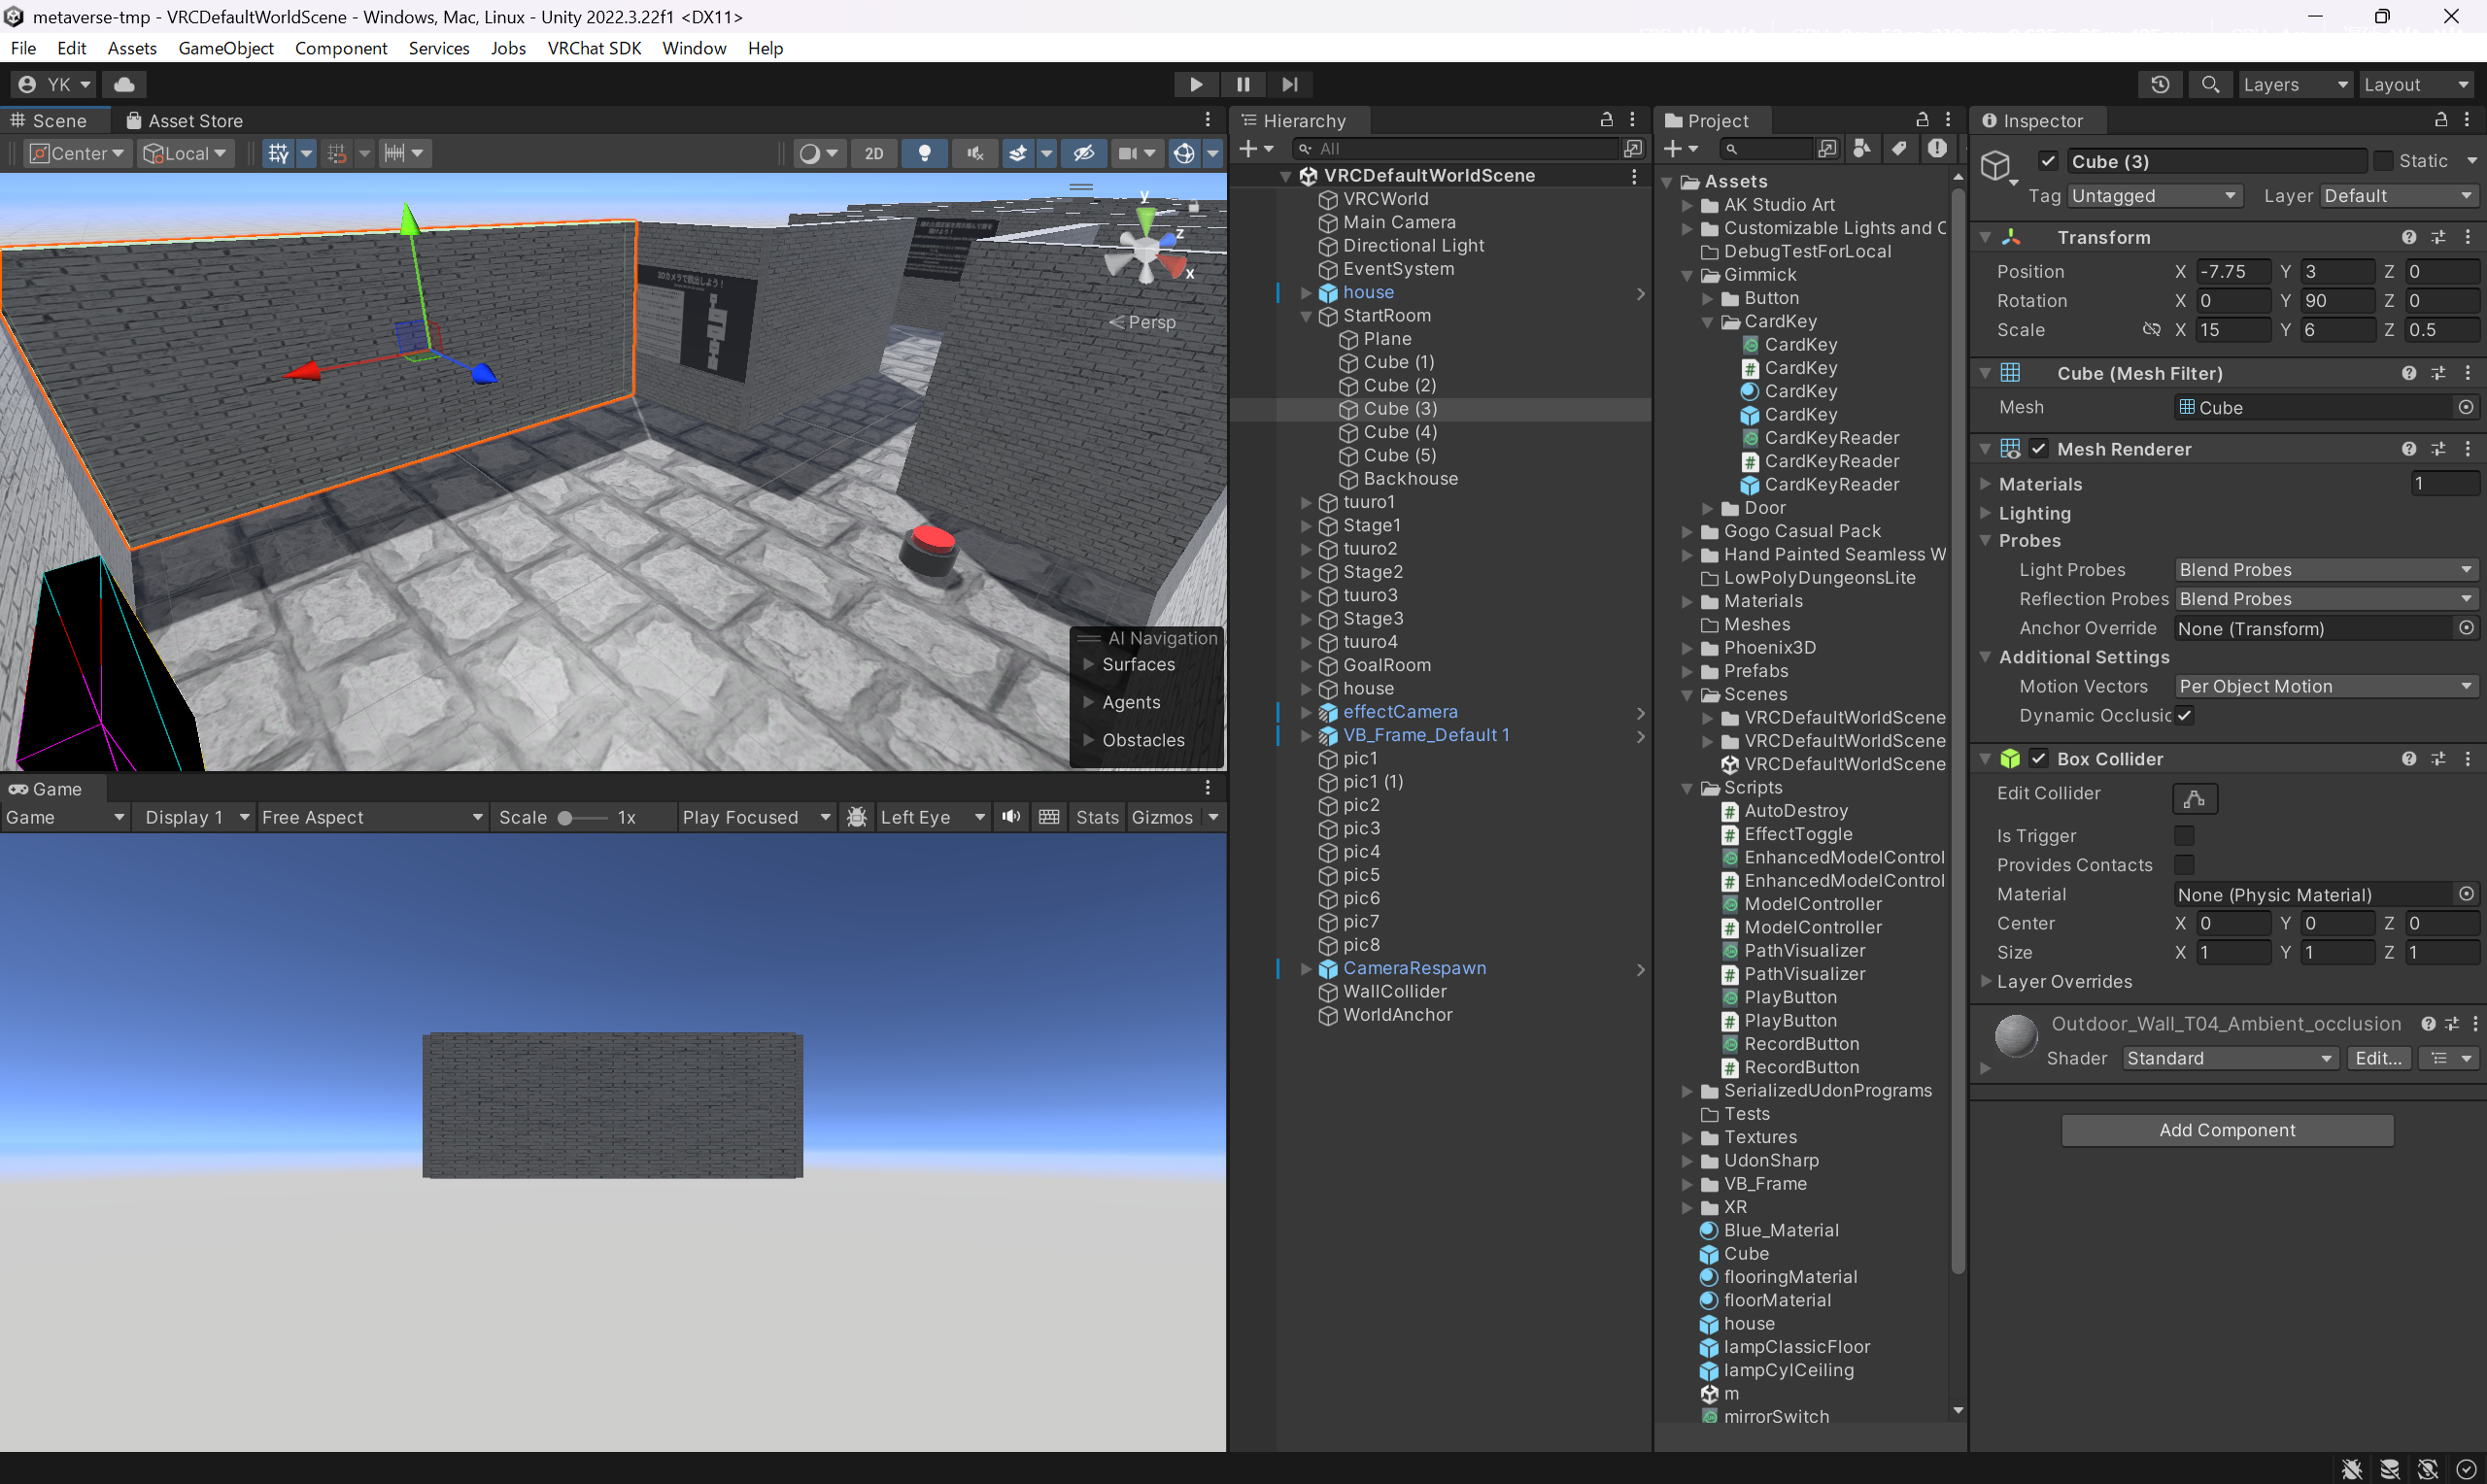
\includegraphics[width=10cm]{unity.png}
    \caption{Unityエディタのリアルタイム編集画面(例)}
    \label{fig:unity_editor}
\end{figure}
例えば6つのboxで小屋を作るときに、Unity等のゲームエンジンの場合は、視覚情報を頼りに座標を決定できる一方で、OpenGLの場合は数値情報を頼りに座標を決定しなければならない。
これらは開発効率に大きな影響を及ぼすと考える。

例えば今回作成した3D空間の実行時間は次のようになった
\begin{table}[H]
    \centering
    \caption{プログラム実行時間}
    \label{tab:execution_time}
    \begin{tabular}{lr}
    \toprule
    種別 & 時間 \\
    \midrule
    real & 0m2.629s \\
    user & 0m5.397s \\
    sys  & 0m0.365s \\
    \bottomrule
    \end{tabular}
\end{table}
このことから、一回の実行に最低でも0.5秒かかり、これを繰り返すことで、数十分のロスが発生することがわかる。
















\end{document}
